% Options for packages loaded elsewhere
\PassOptionsToPackage{unicode}{hyperref}
\PassOptionsToPackage{hyphens}{url}
%
\documentclass[
]{article}
\usepackage{lmodern}
\usepackage{amssymb,amsmath}
\usepackage{ifxetex,ifluatex}
\ifnum 0\ifxetex 1\fi\ifluatex 1\fi=0 % if pdftex
  \usepackage[T1]{fontenc}
  \usepackage[utf8]{inputenc}
  \usepackage{textcomp} % provide euro and other symbols
\else % if luatex or xetex
  \usepackage{unicode-math}
  \defaultfontfeatures{Scale=MatchLowercase}
  \defaultfontfeatures[\rmfamily]{Ligatures=TeX,Scale=1}
\fi
% Use upquote if available, for straight quotes in verbatim environments
\IfFileExists{upquote.sty}{\usepackage{upquote}}{}
\IfFileExists{microtype.sty}{% use microtype if available
  \usepackage[]{microtype}
  \UseMicrotypeSet[protrusion]{basicmath} % disable protrusion for tt fonts
}{}
\makeatletter
\@ifundefined{KOMAClassName}{% if non-KOMA class
  \IfFileExists{parskip.sty}{%
    \usepackage{parskip}
  }{% else
    \setlength{\parindent}{0pt}
    \setlength{\parskip}{6pt plus 2pt minus 1pt}}
}{% if KOMA class
  \KOMAoptions{parskip=half}}
\makeatother
\usepackage{xcolor}
\IfFileExists{xurl.sty}{\usepackage{xurl}}{} % add URL line breaks if available
\IfFileExists{bookmark.sty}{\usepackage{bookmark}}{\usepackage{hyperref}}
\hypersetup{
  pdftitle={One if by land, and two if by sea: Cross-domain contests and the escalation of international crises},
  hidelinks,
  pdfcreator={LaTeX via pandoc}}
\urlstyle{same} % disable monospaced font for URLs
\usepackage[margin=1in]{geometry}
\usepackage{longtable,booktabs}
% Correct order of tables after \paragraph or \subparagraph
\usepackage{etoolbox}
\makeatletter
\patchcmd\longtable{\par}{\if@noskipsec\mbox{}\fi\par}{}{}
\makeatother
% Allow footnotes in longtable head/foot
\IfFileExists{footnotehyper.sty}{\usepackage{footnotehyper}}{\usepackage{footnote}}
\makesavenoteenv{longtable}
\usepackage{graphicx,grffile}
\makeatletter
\def\maxwidth{\ifdim\Gin@nat@width>\linewidth\linewidth\else\Gin@nat@width\fi}
\def\maxheight{\ifdim\Gin@nat@height>\textheight\textheight\else\Gin@nat@height\fi}
\makeatother
% Scale images if necessary, so that they will not overflow the page
% margins by default, and it is still possible to overwrite the defaults
% using explicit options in \includegraphics[width, height, ...]{}
\setkeys{Gin}{width=\maxwidth,height=\maxheight,keepaspectratio}
% Set default figure placement to htbp
\makeatletter
\def\fps@figure{htbp}
\makeatother
\setlength{\emergencystretch}{3em} % prevent overfull lines
\providecommand{\tightlist}{%
  \setlength{\itemsep}{0pt}\setlength{\parskip}{0pt}}
\setcounter{secnumdepth}{5}
\usepackage{tikz}
\usepackage{pgfplots}
\pgfplotsset{compat=newest}
\usetikzlibrary{plotmarks}
\usetikzlibrary{arrows.meta}
\usepgfplotslibrary{patchplots}
\usepackage{grffile}
\usepackage{caption}
\usepackage[utf8]{inputenc}
\usepackage[doublespacing]{setspace}
\usepackage{float}
\usepackage{multirow}

\title{\singlespacing One if by land, and two if by sea: Cross-domain contests and the escalation of international crises}
\author{J Andr\(\'{e}\)s Gannon\footnote{Email: \texttt{jagannon@ucsd.edu}. Web: \texttt{jandresgannon.com}. \newline This version prepared for the 2021 International Studies Association (ISA) annual conference. The author wishes to thank Erik Gartzke and Jon Lindsay who were Principal Investigators on Office of Naval Research Grant N00014-14-1-0071 and the Department of Defense Minerva Research Initiative grant that organized the data collection for this project. Rex Douglass and Thomas Leo Scherer are responsible for the underlying ontology and event data and ICB project managers Jonathan Wilkenfeld and David Quinn oversaw the coding effort. Tom Brailey, David McCrum, James McCullough, Cole Reynolds, Cailen Rodriguez, Woong Suh, and Erin Werner provided excellent research assistance. The author is also grateful for constructive feedback from Shannon Carcelli, Austin Carson, Jasen Castillo, James Fowler, Patrick Hulme, Igor Kovak, Kendrick Kuo, Brian Lai, David Lake, Nicole Letourneau, Saadia Pekkanen, Sara Plana, Laura Resnick Samotin, Branislav Slantchev, Rachel Schoner, Sanne Verschuren, Barbara Walter, and workshop participants at UC San Diego and the Charles Koch Foundation working groups. Previous versions were presented at the 2017 Peace Science Society (International) conference and 2018 International Studies Association conference. Any opinions, findings, or recommendations do not necessarily reflect the view of the Office of Naval Research. Data and code for the empirical analysis can be found at \texttt{https://github.com/CenterForPeaceAndSecurityStudies/icb}.}\\
Department of Political Science\\
University of California, San Diego}
\date{April 8, 2021}

\begin{document}
\maketitle
\begin{abstract}
\singlespacing Speculation is growing that new domains of human endeavor and interaction have begun to trigger important changes in the nature of conflict. Technological advances have added cyber and space to more traditional domains of conflict (land, sea, air). Leading arguments, and anecdotes, suggest increasing competition across domains. Yet, empirical studies are largely constrained to single domains, limiting our collective ability to assess how domains interact. This study uses a new dataset of the domains in which states took military action during 412 international crises from 1918 to 2010 to test existing claims about cross-domain deterrence and cross-domain conflict. Far from being rare, these data show that cross-domain interactions are the modal form of conflict. Indeed, cross-domain conflict is no more frequent (proportionately) today than in decades past. Crises with cross-domain military interactions are also less violent and of no greater duration than crises involving belligerents using similar means. \linebreak \linebreak Word count (excluding references) 9674
\end{abstract}

\hypertarget{introduction}{%
\section{Introduction}\label{introduction}}

Increased technological sophistication has given rise to new modes of conflict as states, organizations, and even individuals have a growing number of ``levers'' or options through which to confront one another. These hostile interactions can take place symmetrically (like for like, within domain) or asymmetrically (``apples vs.~oranges,'' across domain). Recent international crises in particular seem to demonstrate that asymmetric conflict is on the rise and may be a characteristic feature of a new era of conflict. Adversaries seem to be increasingly likely to respond to their opponent's military actions with dissimilar means. Hamas' cyber attacks in 2019 were met with Israeli airstrikes (Newman 2019), Azerbaijani tanks clashed with Armenian drones in 2020 in the Nagorno-Karabakh region (Dixon 2020), Chinese malware attacks have recently joined the fray in an ongoing border skirmish with India (Sanger and Schmall 2021), and Russian electoral inference in 2016 was met with no concrete response due to concerns about the appropriateness of various kinetic and non-kinetic military operations (Healey 2018). There is little consensus about whether to sound the alarm about dangerously escalatory cross-domain interactions (Dixon 2020) or to caution against excess concern (Borghard and Schneider 2019). There also remains considerable ambiguity about whether recent cases of cross-domain conflict are emblematic of the future of warfare (Gatopoulos 2020), or whether they are at most variations on a more durable set of themes (Gannon et al. 2021). As always with assessments of behavior, the question is ``how new is new''?

While recent events have motivated a growing interest in understanding the settings in which states take military action and the consequences those choices have for international stability, the larger context of cross- or multi-domain conflict has not been studied systematically. Part of this is due to difficulty identifying military domains --- is it simply geographic distinctions between land, air, and sea that match up with different military commands? Where do new tools or technologies like nuclear, space, and cyber fit into this typology? The second difficulty concerns limited empirical data concerning the conduct of conflict. While scholars have developed numerous detailed datasets of participants, duration, location, and outcome in order to understand the causes and consequences of conflict, empirically-oriented research concerning where contests take place, within which medium or domain, has only recently received attention (Lindsay and Gartzke 2019a). Researchers and analysts typically frame their inquiries around particular emerging technologies with little validation as to the need or appropriateness of their focus (Sechser, Narang, and Talmadge 2019; Horowitz 2020) or operations within individual domains, unable to address more formative questions about how domains interact (Allen and Martinez Machain 2017; Kostyuk and Zhukov 2019; Cunningham 2020).

This paper takes an inductive, data-driven approach to identify spatial and temporal patterns in the military domains in which states operate during conflict as well as the relationship between cross-domain interactions and the intensity and duration of international crises.\footnote{On the decision to approaching new social science data inductively, see Grimmer, Roberts, and Stewart (2021).} Rather than come up with a new typology of military domains, I take a commonly agreed upon understanding shared by practitioners and scholars that contains the traditional domains of land, air, and sea as well as the recent domains of space, cyber, and weapons of mass destruction (WMD).\footnote{While WMD is rarely a distinct military branch and has geographic overlap with the other domains, they do represent a distinct domain in how actors think about them in the international context. My concern here is less to get domains ``right'' than to expose the diversity of options for conflict setting and consider whether this diversity itself has causal significance.} My motivation in gathering data on the conduct of conflict is driven by the recognition that the domains in which states fight are a reflection of actors' goals, priorities, resolve, and capability and subsequently shape important events like the severity and duration of conflict (Lindsay and Gartzke 2020). In doing so, I developed and introduce a novel dataset of the military domains in which 1238 crisis actors operated during 412 international crises from 1918 to 2010. These data expand on the existing virtues of the familiar and well-regarded International Crisis Behavior dataset (Brecher and Wilkenfeld 2000).

My research contains two initial findings that contributing to existing research on the consequences of conflict domains. First, cross-domain conflict is prevalent, but not novel. Some degree of cross-domain military actions occur in 58\% of crises over the past century, with 24\% of crises involving completely dissimilar military actions by belligerents. Moreover that is not a recent phenomenon, as the rate of ``cross-domainness'' has remained more-or-less constant over the past century despite the accumulation of new military domains during that time period. The number of domains (beyond a nominal need for more than one or two) does not itself seem to have triggered a greater reliance on cross-domain operations in crises. Second, crises in which belligerents engage in cross-domain military conflict are less violent and no more durable than crises in which states respond with like-means. This evidence seems to support optimistic interpretations of the effects of cross-domain conflict and mitigate against the fears of some pessimists. While data on the more salient new domains like cyber remains limited at this time, there is insight to be gleaned about cross-domain interactions in more traditional military domains that should help to inform theories of conflict deterrence and spiral as they are being developed to apply to more recent cases.

This paper proceeds in six parts. Section 2 identifies the existing state of the art concerning the domains in which states fight. Section 3 then identifies the theoretical basis underlying both the cross-domain pessimists and optimists, as applied to the intensity and duration of international crises. Section 4 provides an empirical test of these contrasting theories by introducing a novel dataset of the military domains in which states operated during international crises of the past century. Section 5 discusses the implications of these findings for theories of deterrence and the means of conflict, their application to contemporary foreign policy decisions like A2/AD and AirSea battle in East Asia, Russia's ``little green men'' in Eastern Europe, and kinetic responses to cyber attacks in the Middle East, and avenues for future research. Section 6 concludes.

\hypertarget{existing-theories-of-conflict-escalation-and-how-states-fight}{%
\section{Existing theories of conflict escalation and how states fight}\label{existing-theories-of-conflict-escalation-and-how-states-fight}}

The vast array of theorized determinants of conflict escalation -- defined here in terms of its intensity and scope -- are primarily devoted to factors present before a contest occurs (Morgan 1994; Fearon 1995; Powell 1996). Since most wars end with some compromise rather than the total annihiliation of at least one of the warring sides, the actual conduct of conflict, its process, has much to tell us about when conflicts escalate (Gartner 1998; Wagner 2000; Biddle 2005, 2007; Boot 2006) and how long they last (Slantchev 2004).

There is a well developed literature on how different \textit{ways} conflicts are fought might influence conflict escalation.\footnote{The conduct and consequences of conflict has also been linked to one another since various states characteristics influence the militaries they choose to develop (Kennedy 1976, 177--204).} The ways in which militaries fight influences war's participants (Fordham 2004; Beckley 2017), victors (Rosen 1991; Lyall and Wilson 2009; Cappella Zielinski and Grauer 2020), costs (Caverley 2014), severity (Talmadge 2019; Gartzke and Lindsay 2020), location (Schilde 2017; Crisher 2017), and duration (Martinez Machain 2015; Cappella Zielinski 2016; Caverley and Sechser 2017) as well as what states are able to project power (Corbett 1911; Beasley 2015), what issues are resolved with force (Allison and Morris 1975; Becker 2017; Fearon 2018; Sechser, Narang, and Talmadge 2019), what threats are credible (Buzan and Herring 1998; Slantchev 2003; Post 2019; Montgomery 2020), the efficacy of states' reputation (Erickson 2018), and the balance of power (Glaser 1992; Horowitz 2010; Gartzke, Kaplow, and Mehta 2014).

Despite interest in the means by which state engage in conflict, there is little agreement about how to conceptualize and categorize those means. One broad framework for considering different means of conflict is in terms of the domains in which conflicts take place. There are many ways of thinking about domains, as they can be distinguished from one another by technology, tactic, geography, or purpose (Lindsay and Gartzke 2019a). Some have questioned the utility of conceptualizing these domains as distinct, especially as new domains like space and cyber increasingly play the role of supplementing rather than supplanting operations in the more traditional domains (Stallone 2009; Caton 2012; Libicki 2012). Rather than engage in ontological debates about the best way to typologize conflict behavior, I take domains here as a useful starting point for thinking about differences in the ways that nations choose to fight, and how these differences affect observable attributes of conflict, such as duration or intensity. We know that practitioners think about these domains as distinct and we have theories about the advantages and disadvantages of taking military action in each of these domains (Lindsay and Gartzke 2019a). As already noted, I use the term ``domain'' here loosely to refer to land, air, sea, WMD, space, and cyber.\footnote{International actors certainly also interact through these domains in non-military ways. Some research thinks about this more broadly, where military interactions represent one aspect of interaction, along with economic or diplomatic interactions, for example. The goal here is to contribute to research that disaggregates the military domain, leaving for later larger questions of its integration and impact on other forms of interaction. For existing work on issue linkages involving military and non-military domain interactions, see Rosenau (1968), Tollison and Willett (1979), Vasquez (1983), Morgan (1990), Morgan and Palmer (2000), Starr (2000), Poast (2012), Greenhill (2019), and Huang and Kang (2019).} Domains differ from one another in how political actors think about them, the constraints (and opportunities) they offer concerning power projection capabilities, movement, coordination, casualty risk, and cost (Lindsay and Gartzke 2020, 9--10).\footnote{There are differences in the strengths and weaknesses of capabilities that produce unique cross-domain dynamics regarding conflict intensity and duration (Lindsay and Gartzke 2020). A more discrete analysis would involve the separate ``tools'' or platforms used to fight in different domains (tanks or artillery are different from airplanes or helicopters, etc.). Such an approach would require an extremely detailed theorizing and data collection effort, with possibly only a modest increase in insight Still, the current analysis may be seen as a ``proof of concept'' for this more detailed inquiry, showing that disaggregating capabilities adds useful empirical content.}

If the problem of the security dilemma is to decide whether a particular response to an adversary's behavior will deter or escalate, the problem as applied to the conduct of conflict is whether the military means one chooses determine the likelihood of escalation. Snyder (1965, 187) described the importance of new (nuclear) means and escalation long ago. ``{[}N{]}uclear technology introduced a new form of intent-perception and a new form of uncertainty --- that concerning what types of military capability the opponent was likely to use and what degree of violence he was willing to risk or accept''. This view is widely credited with originating discussion of the stability-instability paradox regarding the relationship between capabilities an actor possesses and the capabilities they use. The resulting debate created competing perspectives on escalation, characterized as deterrence and the spiral model. Snyder's deterrence perspective contrasts with the spiral model espoused by Jervis (1984). Powell (2015)'s recent work represents the newest attempt to theorize the relationship between power and risk. He develops a formal model where the challenger decides how much military power to use to achieve its ends. The more power it uses, the higher its chance of winning, but the higher the potential risk of escalation as well. Although an important contribution to understanding conflict escalation and the deterrence and spiral models of conflict, what it means to bring ``more power to bear'' in a crisis is unspecified (Powell 2015, 598).

Just as the quantity of capabilities a state devotes to a contest is likely to influence its outcome, the qualities of those capabilities may also matter in shaping the content and characteristics of the conflict (Carcelli and Gartzke 2017). One might claim with a reasonable degree of plausibility that different military domains have different inherent level of belligerence that can be compared with one another. A nuclear strike is likely to be interpreted as a more intense form of military violence than a non-nuclear attack, even if the effects in both cases are largely comparable (Tannenwald 1999). Yet this intuition remains coarsely formulated and may even prove empirically problematic, due to multi-causality, strategic interaction, and other factors. Foundational escalation metaphors, such as ``ladders'' (Kahn 2007) often parallel the distinction of domains, making separating out cause and coincidence more difficult. Libicki (2009, 28--29), for example, notes that belligerence increases as an actor shifts from diplomatic and economic to cyber, then physical force, then nuclear force. But whether such patterns are more indicative of the effects of the form of competition or of the intentions of competitors remains unclear. Escalation may or may not be associated with whether responses are symmetric or asymmetric. Whether the move from one ``physical force'' domain to another is consistent with the deterrence or spiral model of conflict remains to be shown.

With these issues in mind, evaluations of the importance of actions in domains has recently shifted to theorizing about interactions across domains (Lindsay and Gartzke 2019b). There is suspicion that cross-domain interactions are more prevalent now because there are more (and newer) domains in which states can operate. While study on the nuclear domains and conventional-nuclear interactions is no longer in its infancy (Kissinger 1960; Wallace 1979; Weede 1980; Carver 1986), this has recently expanded to cross-domain or multi-domain interactions involving newer domains of space (Early 2014; Lin-Greenberg and Milonopoulos 2021), cyber (Healey 2018; Libicki 2012; Nye 2017; Schneider 2017; Lindsay and Gartzke 2018; Kostyuk and Zhukov 2019), drones (Boyle 2013; Byman 2013; Hazelton 2016; Horowitz, Kreps, and Fuhrmann 2016; Schneider and Macdonald 2017; Zegart 2018), artificial intelligence (AI) (Horowitz 2018; Jensen, Whyte, and Cuomo 2020; Johnson 2020), and quantum computing (Lindsay 2020; Gamberini and Rubin 2021). Both researchers and policymakers have expressed concern that these and other new tools of warfare may strengthen or embolden revisionist forces in world affairs, (Brands 2016), although skepticism about the novelty and efficacy of these ``new'' forms of warfare has also cast some doubt on those concerns (Gannon et al. 2021).

Empirical evidence, however, remains limited due in large part to the very novelty and putative heterogeneity of these emerging domains (Horowitz 2020). Even where recent empirical research has made headway in identifying the ownership and use of new modes of warfare like satellites (Early 2014; Early and Gartzke 2021), cyber attacks (Valeriano and Maness 2014; Borghard and Lonergan 2017; Kostyuk and Zhukov 2019), drones (Horowitz, Kreps, and Fuhrmann 2016), and smart bombs (Kahn and Horowitz 2021), the efforts are contained to a single capability or domain. As a result, existing research on cross-domain conflict tends to approach the ``cross'' component of the subject in terms of within-actor behavior, rather than across actors. As Nye (2017, 46) notes, ``it is a mistake to see the cyber realm in isolation. The term ``cyber deterrence'' can be confusing because theorists tend to focus on in-kind or in-domain deterrence rather than on a broad range of tools that can be used both actively and passively and with graduated effects. A response to a cyberattack need not be by cyber means any more than a response to a land attack need be by the army rather than naval or air forces."

I agree with Powell (2015, 598) when he writes that ``the amount of power the challenger brings to bear affects the stability of the conflict.'' I expand upon his conceptualization of the military might used by the challenger. Powell varies the amount of power --- what he terms ``military might'' --- as different types or levels of conflict (Powell 2015, 599). But types and levels of conflict are not synonymous, nor should they be grouped together (Kreps and Schneider 2019). I seek to provide insight about how the relationship between the \textit{types} of conflict exercised by adversaries explains differences in conflict escalation.

\hypertarget{the-dialectic-across-domains}{%
\section{The Dialectic Across Domains}\label{the-dialectic-across-domains}}

``A ship's a fool to fight a fort.''\footnote{The quote is generally (mis)credited to Admiral Lord Horatio Nelson, RN (Ferreiro 2016).} But is it wiser for a commander, or a nation, to attack a fort with a fort? Interpreting ``foolish'' actions as those that escalate a conflict in terms of violence and/or duration, perhaps unnecessarily, I identify two sets of disparate expectations about cross-domain interactions. Despite the contrasting predictions in the literature best characterized by the classical dialectical debate between deterrence theory and the spiral model, both perspectives share the assumption that the manner in which states engage in a crisis influences whether it is resolved peacefully or violently. These perspectives thus differ in whether demonstrations of resolve and/or capability succeed or fail when they involve transporting actions to a military domain in which one's opponent is not currently operating.

\hypertarget{cross-domain-escalation-the-danger-of-taking-an-ear-for-an-eye}{%
\subsection{Cross-domain escalation: the danger of taking an ear for an eye}\label{cross-domain-escalation-the-danger-of-taking-an-ear-for-an-eye}}

Crises in which actors interact in dissimilar military domains may be more violent and/or last for a longer period of time because cross-domain interactions complicate interpretations of proportionality and the scope of disputed stakes, thus contributing to misinterpretation of resolve (Morrow 2019). If a belligerent taking action with 100 ground troops is met with the defender deploying 200 ground troops, the belligerent could reasonable interpret the defender's action as a ``re-raise'' indicating the defender places a high value on the issue(s) in dispute. But if the defender responds to a deployment of 100 troops with 5 aircraft, it is less clear whether that is a re-raise, or instead is an effort to achieve something different, such as saving face. In essence, cross-domain conflict presents actors with an apples to oranges comparison, making it more difficult to assess relative resolve or an opponent's value for the issue(s) at stake. This injection of (additional) ambiguity arguably makes a negotiated settlement more difficult by clouding evaluations of the bargaining range.

Uncertainty can cause, or worsen, a contest by creating incompatible expectations about a contest's likely outcome or utility (Fearon 1995; Gartzke 1999). Asymmetry in the military domains in which belligerents are taking actions can be a source of that uncertainty. Cross-domain interactions may be perceived by the adversary as shifting to a domain where one has escalation dominance because you highly value the stakes of the conflict. Since each military domains has different strengths and weaknesses concerning outcomes like credibility, relative war fighting ability, costs, and signaling, operating in a different domain that your adversary may signal a difference in one's tolerance for cost and risk (Carcelli and Gartzke 2017; Gartzke et al. 2017; Lindsay and Gartzke 2019a). One can represent this aspect of military domains in terms of a game of rock, paper, scissors, where each domain's characteristics bring advantages against some of your opponent's chosen domains, but disadvantages against others (Lindsay and Gartzke 2019a, 16). In discussing the dangers of Chinese power projection from land, former US National Security Adviser H.R. McMaster (2016) advised practitioners ``recognize that synergy, right, between joint force capabilities and how, you know, really joint operations - it's rock, paper, scissors, you know? So if you can - if you have all of those tools available - maritime, aerospace, cyberspace, land capabilities - then you're able to pose that enemy with multiple dilemmas.''

While presenting your enemy with multiple dilemmas --- responding to your adversaries ``rock'' with ``paper'' --- may help you win the conflict, it could also produce an incentive for your opponent to do the same --- respond with ``scissors'' (and so on) --- thus encouraging escalation. Responding in-kind --- playing rock against rock --- may be de-escalatory because it represents a symbolic gesture to opt against one's comparative advantage, one's most efficient response (paper), that would require the opposing side to engage in a new, more efficient response (scissors), etc.\footnote{A similar argument about the defense-dominant nature of responding in-kind is made by Biddle and Oelrich (2016).} Responding in-kind thus represents a symbolic gesture to opt against an efficient response that would require the opposing side to engage in a new more efficient response. By responding in-kind, states can agree to call it a draw in a way that represents a compromise (Carson 2016, 2018; Carnegie and Carson 2018). Conversely, undertaking that engagement in a new military domain may unintentionally create an ``escalatory updraft'' if the opponent misinterprets what should be a tit-for-tat response that ends aggression with one that instead escalates it (O'Neill 1991, 104). To return to Powell (2015)'s logic about bringing more power to bear, taking action in a new domain may represent a reduction in cost for you, but the very logic of escalation dominance that generates that outcome also means interacting in the new domain represents an increase in cost for your opponent, with adverse consequences for the likelihood of a peaceful settlement. Cheap and easy can be attractive, but it sends mixed messages. An opponent may be cowed by superior capabilities across domains, but they may also be encouraged by limited evidence of an opponent's willingness to pay the high price of a larger contest.

~~\textbf{\textit{Pessimist Hypothesis:}}\textit{ Interstate crises in which belligerents act in dissimilar military domains should be more violent and longer in duration than those in which belligerents act in similar military domains.}

Scholars have raised this concern in the context of the US and China in arguing ``A war at sea could thus quickly become a war on land, potentially even raising risks of nuclear escalation if the US starts to erode potential capabilities relevant to China's nuclear arsenal'' (Talmadge 2019, 880--81).\footnote{See also Talmadge (2017) and Cunningham (2020) for more on China and the risk of nuclear escalation.} States often share an assumption that opponents will ``follow precedent by responding in kind with similar weapons against a similar target set'', so failing to do so risks un-calibrated escalation (Warden 2018, 24). In the cyber context, scholars have argued retaliating to physical force with a cyber attack may raise issues of proportionality (Libicki 2009). While China thinks that cyber attacks are a proportional response to US trade pressure given the stakes each place on the sectors being harmed by the other actions, the United States disagrees. ``The U.S. approach to Chinese gray zone tactics seems to be consistently several steps behind the threat. As in the Russia case, this is likely due in large part to the absence of a coherent strategic approach, leading to ad hoc U.S. responses from one crisis point or domain of interaction to the next.'' (Hicks and Friend 2019, 8).

\hypertarget{cross-domain-deterrence-the-safety-of-playing-chess-while-your-opponent-is-playing-checkers}{%
\subsection{Cross-domain deterrence: the safety of playing chess while your opponent is playing checkers}\label{cross-domain-deterrence-the-safety-of-playing-chess-while-your-opponent-is-playing-checkers}}

Just as deterrence and the spiral model make contrasting claims from similar priors, the opposite (optimist) logic could also be at play in assessing cross-domain escalation. Crises involving states taking military actions in dissimilar domains could be less likely to escalate by communicating a change in the stakes and a willingness to escalate or by giving one side the upper hand if conflict actually breaks out (Rovner 2020). The apples to oranges analogy may be backwards; rather than creating confusion about resolve and the opponent's evaluation of the stakes, a willingness to play a different game entirely may sharpen that logic in a way that signals it may be better to try to resolve the conflict without fighting.

Rather than simply thinking of military domains as playing rock, paper, or scissors, the virtues of different domains in their ability to signal or fight wars also creates distinctions in what it means to ``play'' one of them. Threats differ from forward deployments which are further different from seizing territory or discharging a rocket (Lai 2004; Mackey 2014; Post 2019). In this way, operating in a new domain could deter rather than inflame by providing an avenue to graduated escalation (Cashman and Robinson 2007; Montgomery 2020). Reinforcing an army unit by putting bombers on alert or forward deploying a naval unit could be a graduated way of signaling resolve and a willingness to escalate without necessarily increasing the number of army troops already on the battlefield (Slantchev 2005, 2011; Warden 2020). Using the same assumption of escalation dominance, action in a new domain in which your opponent is not operating because they do not have escalation dominance in that domain can be a costly signal that makes a negotiated settlement more likely (Cimbala 1994; Quek 2013; Handberg 2016). In the same way that children on a playground may yell `hotter' or `colder' as their blindfolded classmate tries to find some object, operating in new domains can add credibility to verbal statements about whether an actor perceived an offered negotiation as preferable to continuing to fight. Furthermore, deterrence may work not because of mutual vulnerability, but because of one-sided fear about overwhelming punishment (Green 2020; Lieber and Press 2020). If operating in a new domain during a crisis is indicative of a state's willingness to take action in a domain where they have escalation dominance, that may convey to the other side that the state is willing to incur a higher cost.

~~\textbf{\textit{Optimist Hypothesis:}}\textit{ Interstate crises in which belligerents act in dissimilar military domains should be less violent and shorter in duration than those in which belligerents act in similar military domains.}

Historically, Nixon placing bombers on nuclear alert during the 1969 Giant Lance operation demonstrated the introduction of a new domain as a way to signal a willingness to gradually escalate or de-escalate based on their opponent's actions (Sagan and Suri 2003; Burr 2005). This case is consistent with existing theories of signaling in finding that some domains are better suited to turning the dial incrementally rather than all at once (Kroenig 2018; Post 2019; Montgomery 2020). President Kennedy had a similar rationale behind the ``flexible response'' doctrine in 1961, which aimed to provide more options for controlled escalation. In the event of more limited Soviet aggression like an attempt to hold Berlin hostage, proponents of flexible response hoped the more credible threat of responding with other conventional forces would be sufficient to get the Soviet Union to back down (Duffield 1991).\footnote{There is disagreement concerning whether Kennedy actually believed in --- and would have implemented --- ``flexible response'' in the ways espoused at the time or if it merely served political purposes (Gavin 2001). I use this example here to illustrate the strategic logic held by proponents of the policy, regardless of whether or not the United States would have actually followed through.} Similarly, a ceasefire was declared between Israel and Hamas the day after Israel responded to Hamas' cyberattacks with an airstrike (Morris, Eglash, and Balousha 2019). One way to interpret this event is the very conditions that make a cross-domain response a threat of immediate escalation make it conducive to medium and long-term de-escalation. By showing that an opponent has crossed a red line in the intensity of their aggression, an unexpected cross-domain response could convey that there are significant costs to be had if they do not pull back (Altman 2018).

As an aside, cross-domain interactions may not be the direct cause of escalation (or de-escalation), but rather an observable indicator for different motives to escalate in a way that masks the stakes (Slantchev 2011). States with more at stake may be more willing to escalate, but cross-domain interactions may communicate that poorly since it relies on your opponent identifying the costs of your action when that same action would generate different costs for them.\footnote{For existing research on motives for escalation, see Lebow (2010), Dafoe, Renshon, and Huth (2014), Paul, Larson, and Wohlforth (2014), Fikenscher, Jaschob, and Wolf (2015), Renshon (2016), Lupton (2018), and Shifrinson (2019).} Rather than try to empirically identify whether the underlying causes of cross-domain interactions are directly or indirectly determinants of conflict intensity, I simply hope to shed light on the association between the use of these domains --- whatever their origins --- and crisis outcomes.

\hypertarget{empirics}{%
\section{Empirics}\label{empirics}}

\hypertarget{research-design}{%
\subsection{Research Design}\label{research-design}}

The study's primary empirical contribution is the creation of a new dataset detailing the domains in which military actions or conflict occurred during 412 distinct crises from 1918 to 2010. In sum, the new data contains information on 1238 crisis actors, the majority of which are states.\footnote{International organizations and non-state actors are often involved in crises and sometimes deploy military or quasi-military capabilities like peacekeepers or foreign aid distributors. I do not consider the military logic of these actors here, but the data is available for future work on the topic and includes 3833 actors that played some role in an international crisis.} This crisis-domain dataset represents -- to the best of my knowledge -- the most extensive data collection available on the domains in which militaries operate during conflict.

Doing so involved three distinct steps. First, a research team event coded the 412 crises in the International Crisis Behavior (ICB) dataset (Brecher and Wilkenfeld 2000; Brecher et al. 2020), identifying the military domains in which crisis actors acted at the sentence level. Second, I re-organized and subset that data to the crisis-dyad level using pre-existing work on ICB crisis-dyads. Third, I create a new measure of the dissimilarity of the domains in which each side in the crisis took military actions, an ordinal attribute of domains that I refer to as ``cross-domainness''. I discuss each of these steps in greater detail below.

\hypertarget{event-coding}{%
\subsubsection{Event coding}\label{event-coding}}

A research team extended the ICB dataset by gathering extensive data on how actors interacted during crises. The ICB dataset provides a unique opportunity to examine conflict escalation because it is not limited to cases where conventional military conflict occurred. Rather, the data examines crises --- some of which were militarized and others which were not. This provides variation in the dependent variable since I can compare cases where a crisis did violently escalate to cases where the crisis did not. The dataset introduced here contains detailed information on the military domains used by each actor during every international crises. As such, the unit of analysis is the crisis-actor and the newly coded variables are binary values representing whether that actor employed a given domain during the crisis.

The data source used by the coders was the ICB crisis narratives that provide qualitative descriptions of each crisis. This has a few benefits over other events datasets. First, the ICB crisis narratives are written in a systematic fashion. They are each of comparable length, contain the same level of detail, and were written by the same research team at the University of Maryland. This reduces concerns that variation among crisis variables is due to variation in the measurement process. For example, more recent crises do not have more detailed crisis narratives which is not the case for the reporting of militarized interstate disputes captured by scraping news sources. Second, the ICB narratives are accompanied by the widely-used and well-regarded ICB dataset that codes important international relations variables for numerous aspects of the actors and crises represented in the dataset. This helps verify the coding effort since the information that coders extract from the crisis narratives should be consistent with previous codings that populate the quantitative ICB dataset.

The data created here involves the domains in which states took actions during international crises.\footnote{This is a subset of a broader project producing event data using the ICB narratives. For the complete event data and more detailed explanation of the underlying ontology, see Carcelli et al. (2021).} I define the domains in which a crisis-actor can take a military action based on the military units that undertook the action, as described in Table \ref{tab:domains}. The coders distinguished actions, speech acts, and thoughts for consistency with pre-existing event datasets like CAMEO and Phoenix (Schrodt et al. 2005; Schrodt 2012; Althaus et al. 2020). Actions are defined as physical acts performed by one of more actors. Examples of military actions include raises in alert level, mobilizations, fortification, military exercises, weapons tests, deployments, shows of force, blockades, border violations, attacks, invasions, and bombardments. Planning to take an action does not constitute an action unless this action is subsequently carried out. For example, a state making a verbal threat to send tanks into a neighboring country is not coded as a ground action unless the state mobilized, deployed, invaded, attacked, or otherwise took a subsequent physical action with land units.

\begin{table}[]
\centering
\begin{tabular}{|l|l|}
\hline
\textbf{Domain} & \textbf{Description} \\
\hline
Air & Bombers, fighters, and missiles \\
Cyber & Information operations and cyber disruption \\
Land & Armored vehicles, artillery, and troops \\
Sea & Aircraft carriers, submarines, and surface ships \\
Space & Satellites and surveillance beyond the earth's atmosphere \\
WMD & Nuclear, chemical, and biological weapons \\ 
\hline
\end{tabular}
\caption{Military domains coded for each crisis actor. Codings are binary with 1 indicating the actor took an action in that domain during the crisis and 0 otherwise.}
\label{tab:domains}
\end{table}

The first set of codings were done by graduate students at the University of Maryland that were overseen by the ICB directors who helped construct the original ICB datasets and narratives. For each crisis, two research assistants coded the ICB crisis narratives at the sentence level for a new series of variables. Coders could not make reference to the existing codings and the raw coding includes a measure of uncertainty for each coder. Coders selected one of the 412 ICB crises and for each individual sentence in the corresponding ICB crisis narrative, they coded the events that occurred as a series of actions undertaken by an actor along with supporting details like when the action took place, where, and to what effect. The codings were then double checked, with particular attention paid to the less common domains of WMD, space, and cyber. The final version of the data includes an aggregation of the multiple different codings that exist for each case. This project only focuses on the military domains used during these crises. This represents an improvement over current efforts to analyze aggregate analysis of crisis behavior by including fine-grained information about how actors behaved. Figure \ref{fig:domain-count} shows the distribution of actions taken in each domain by crisis actor. Consistent with expectations, the past century witnessed crisis-actors most often operating in the land domain, with significantly fewer WMD, cyber, and space actions taking place. Even so, the prevalence of WMD events may appear higher than expected. This is because the domain variables refer to where the action took place. This does not refer to what was used during the action, but where the action happened. As a result actions like raising nuclear alert levels or forward deploying nuclear bombers constitute WMD ``actions'' even if nuclear bombs were not subsequently detonated. The low number of space and cyber actions do not reflect the rarity of military action in the space and cyber domains, but rather the rarity of those domains \textit{in international crises}. This distinction is important, as existing work has documented numerous cases of cyber attacks that occur outside the universe of international crises defined by the International Crisis Behavior project (Valeriano and Maness 2014).

\begin{figure}[h!]

{\centering 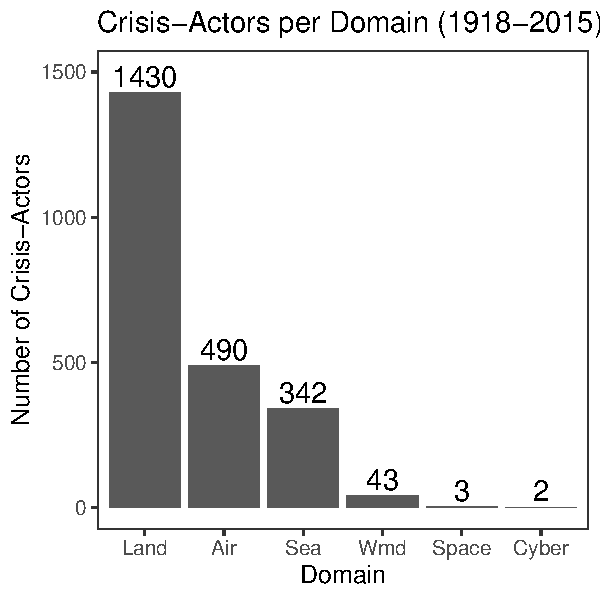
\includegraphics{2021-03-26_ICB-Domains_files/figure-latex/domain-count-1} 

}

\caption{Distribution of domains by crisis-actor}\label{fig:domain-count}
\end{figure}

Of course, actors often fail to contain their military activities in a given crisis to a single domain. Conventional wisdom surrounding the efficacy of full-spectrum military forces rightly lead one to believe that actors often engage in multiple military domains simultaneously, especially as the stakes of a conflict heighten. Figure \ref{fig:domain-combos} describes the combination of military domains that each crisis-actor undertook. While the sole deployment of land forces still remains by far the most common form of military action, combined land- and air operations is the second most common, followed by land, sea, and air being used in unison.

\begin{figure}[h!]

{\centering 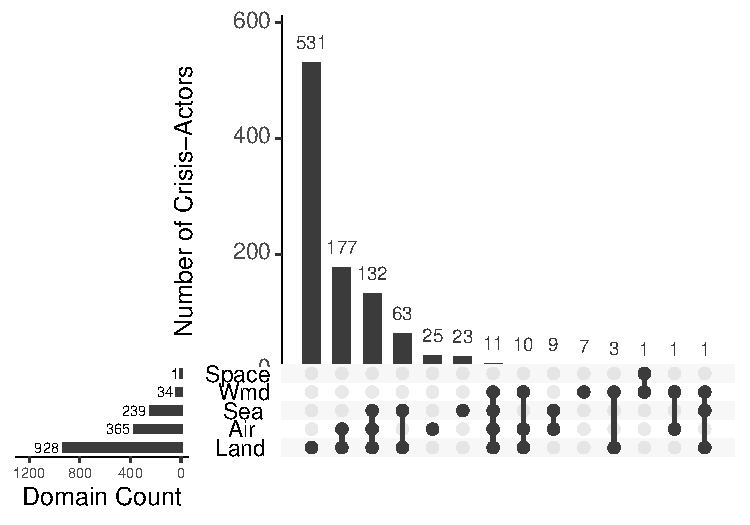
\includegraphics{2021-03-26_ICB-Domains_files/figure-latex/domain-combos-1} 

}

\caption{Combination of domains for each crisis actor. Each bar represents the number of crises with that unique intersection of domain values present}\label{fig:domain-combos}
\end{figure}

\hypertarget{identifying-crisis-dyads}{%
\subsubsection{Identifying crisis-dyads}\label{identifying-crisis-dyads}}

The original ICB data exists at two levels of analysis, the crisis-level and the crisis-actor level. A crisis is defined as an international event that meets 3 conditions. First, an actor must perceive a threat to one or more of its basic values. Second, the actor must have an awareness of a finite timeline for responding to that value threat. And third, there must be a heightened probability of military hostilities. A crisis can escalate to an actual military dispute, but that does not always happen. Many crises are resolved prior to escalation to actual conflict because the existence of the crisis motivates diplomatic solutions to resolve the crisis without resorting to war. While the actor-level data latter contains more granularity, it leaves the role of each actor unspecified. So after identifying the military domains in which crisis-actors took actions, this new data was merged with existing data on ICB crisis-dyads (Hewitt 2003; Beardsley and Asal 2009; Levin-Banchik 2020). Three conditions determine whether an actor is included is the ICB crisis-dyad data. First, both sides of the dyad must be states as defined by the Gleditsch and Ward (1999) state list dataset. Second, at least one state must meet all the crisis conditions specified by the original ICB project. Third, at least one actor must perceive that the other has directed a threat or hostile action against the first actor.

Although the new ICB domains data created for this project contains information on 3833 crisis-actors, not all of them are members of crisis-dyads. After subsetting to the crisis-dyad conditions, I am left with 1238 crisis-dyad actors that were on one of two sides in 412 previously identified crisis-dyads. The 2595 actors on which domain data exists, but are not included in the statistical analysis of crisis-dyads and conflict intensity is primarily attributed to newly gathered information on non-state actors (including international organizations like the Organization of American States and United Nations) or actors that were mentioned in the crisis narratives as a mediator or neighboring state, but not a crisis participant involved as one of the two sides in the crisis. Numerous crises involve multiple dyads if, for example, military coalitions were involved. To simplify coding, when multiple actors participated on the same side in the conflict, that side was coded as having taken actions in a given military domains if any actor on that side took actions in that domain. For example, if both France and the United States were coded as being on the same side (side A) in a crisis and France deployed naval assets and the United States deployed ground forces, side A is simply coded as having taken action in both the naval and land domain.

\hypertarget{measuring-cross-domainness}{%
\subsubsection{Measuring cross-domainness}\label{measuring-cross-domainness}}

The third and final step involves identifying the dissimilarity of the domains in which each side of each crisis-dyad took actions. I call this measure ``cross-domainness'', which is a variable at the crisis level of analysis that is bounded between 0 and 1. For each crisis, if the two sides took actions in identical domains, cross-domainess is low. If the two sides took actions in entirely distinct domains, cross-domainness is high.

I produce this measuring by using a Jaccard similarity coefficient to compare the military domains in which each side in a crisis-dyad operated during each ICB crisis. This measure identifies the union of domains in which each side took actions as a ratio of those in which only one side took action, such that for a crisis-dyad with two sides A and B, \(J_{(A, B)} = \frac{A \cap B}{A + B - (A \cap B)}\). Table \ref{tab:jaccard} provides descriptive examples of how domain similarity in various crises is measured. During North Korea's nuclear test in 2009, North Korea launched a satellite followed by an underground nuclear test. The United States, Japan, and South Korea moved naval forces as a part of military drills and kept interceptor-capable ships in the region following those drills. Since North Korea (side A) took action in the space and WMD domain while the US, South Korea, and Japan (side B) responded in the naval domain, this crisis had an entirely cross-domain interaction -- the two sides took no military action in the same domain. By contrast, the Kashmir crisis that involved India, Pakistan, and China in 1965 only involved land forces being deployed by both sides. India (side A) sent troops across the ceasefire line in response to infiltration by Pakistani ``freedom fighters'' and China (both constituting side B) then responded with troop movements near the border. In this case, the two sides responded exclusively ``in-kind'', so this crisis was entirely within-domain. The Jaccard measure is appropriate because each crisis contains precisely two sides, meaning there are two vectors to compare, the values are binary, and I am concerned with the similarity of measures that were employed as opposed to those that were not. Similar measures like the simple matching coefficient (SMC) are less appropriate because they weigh mutual 0's as an increase in similarity.\footnote{For an overview comparing different similarity measures and criteria for their appropriate application, see Ahlgren, Jarneving, and Rousseau (2003) and Egghe (2010).} These kinds of measures are less appropriate for measuring similarity in military domains since there is variation across space and time about what 0's mean. In some cases, 0's are an omission by choice (states chose not to act in this domain) but in others they represent omission by necessity (states lacked the capacity to act in this domain). Although neither the US nor Vietnam used WMDs during the Vietnam war, that doesn't make their military strategy similar because the US could have done so but did not, while Vietnam could not have. Thus, 0's mean different things. I avoid this problem by measuring similarity in terms of what they did use, in which domain.

\begin{table}[]
  \centering
  \begin{tabular}{|l|l|cccccc|c|}
  \hline
    \textbf{Crisis} & \textbf{Belligerents} & \multicolumn{1}{l}{\textbf{Land}} & \multicolumn{1}{l}{\textbf{Air}} & \multicolumn{1}{l}{\textbf{Sea}} & \multicolumn{1}{l}{\textbf{WMD}} & \multicolumn{1}{l}{\textbf{Space}} & \multicolumn{1}{l|}{\textbf{Cyber}} & \multicolumn{1}{l|}{\textbf{Jaccard}} \\ 
    \hline
    \multirow{2}{*}{N Korea Nuclear IV (2009)} & US, Japan, S Korea & - & - & 1 & - & - & - & \multirow{2}{*}{1} \\
     & N Korea & - & - & - & 1 & 1 & - & \\
    \hline
    \multirow{2}{*}{Yemen War IV (1967)} & Yemen, Egypt & 1 & 1 & - & 1 & - & - & \multirow{2}{*}{0.67} \\
      & Saudi Arabia & 1 & - & - & - & - & - & \\ 
    \hline
    \multirow{2}{*}{Kashmir I (1947)} & India & 1 & 1 & - & - & - & - & \multirow{2}{*}{0.5} \\
      & Pakistan & 1 & - & - & - & - & - & \\ 
    \hline
    \multirow{2}{*}{Gulf of Tonkin (1964)} & S. Vietnam, U.S. & 1 & 1 & 1 & - & - & - & \multirow{2}{*}{0.33} \\
      & N. Vietnam & 1 & - & 1 & - & - & - & \\ 
    \hline
    \multirow{2}{*}{Kashmir II (1965)} & India & 1 & - & - & - & - & - & \multirow{2}{*}{0} \\
     & Pakistan, China & 1 & - & - & - & - & - & \\ 
    \hline
  \end{tabular}
  \caption{Example of cross-domainness measure at the crisis-level using the Jaccard similarity coefficient. The measure is bounded between 0 and 1, with 0 indicating the two sides took actions in identical domains and 1 meaning complete dissimilarity.}
  \label{tab:jaccard}
  \end{table}

Figure \ref{fig:cddness} represents the distribution of cross-domainness for all ICB crises. This figure demonstrates that cross-domain military crises are not unusual, just the opposite. Cross-domain conflict behavior represents the modal form of conflict interaction in crises over the past century. Of the 412 ICB crises, 24\% are entirely cross-domain, meaning the two side had zero overlap in what military domains they operated in during the crisis, and 58\% had at least some amount of cross-domain interaction. In only 42\% did both sides behave in-kind. Figure \ref{fig:cddness-time} shows that the temporal trend of cross-domain interactions runs contrary to conventional wisdom. Despite the common demarcation of the nuclear age and advent of new domains like cyber and space, cross-domain conflict is not an emerging property of new, technological conflict domains (at least not within crises). Although new military tools have become available to states at an arguably ever greater pace, they have not led to an increase in cross-domain activities. Either these domains are not being utilized in international crises, or they are being utilized in about the same way that older domains of conflict were and continue to be exercised. There is no evidence in these data of a transformation of military affairs related to cross-domain conflict. Rather, cross-domain conflict has been, and continues to be, a common feature of conflict behavior generally, at least within crises.

\begin{figure}[h!]

{\centering 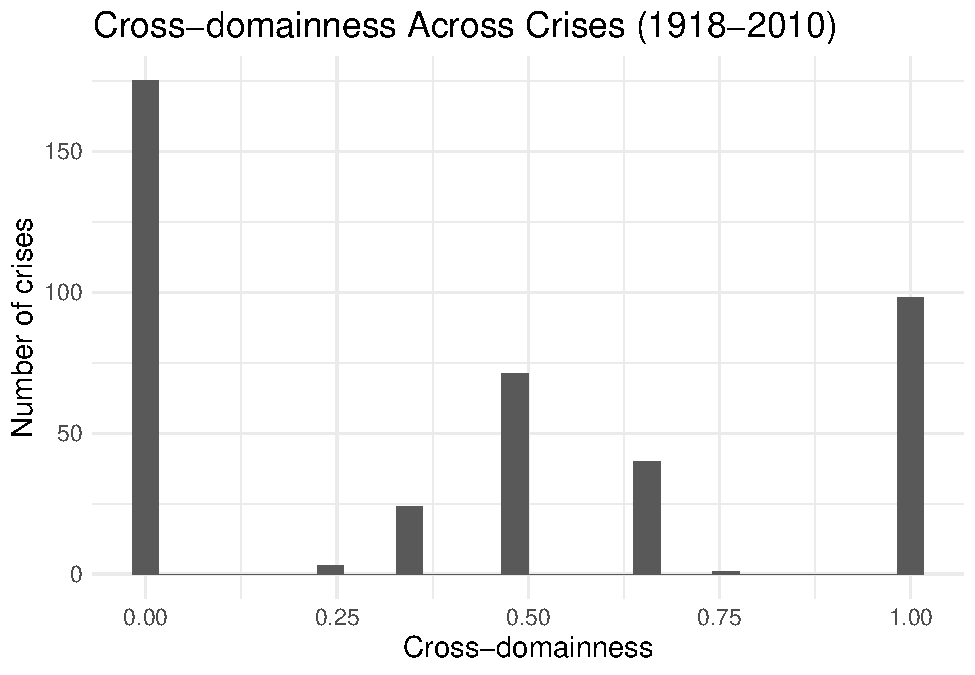
\includegraphics[width=0.8\linewidth,]{2021-03-26_ICB-Domains_files/figure-latex/cddness-1} 

}

\caption{Distribution of cross-domainness in international crises. Higher values represent higher cross-domain interactions between adversaries}\label{fig:cddness}
\end{figure}

\begin{figure}[h!]

{\centering 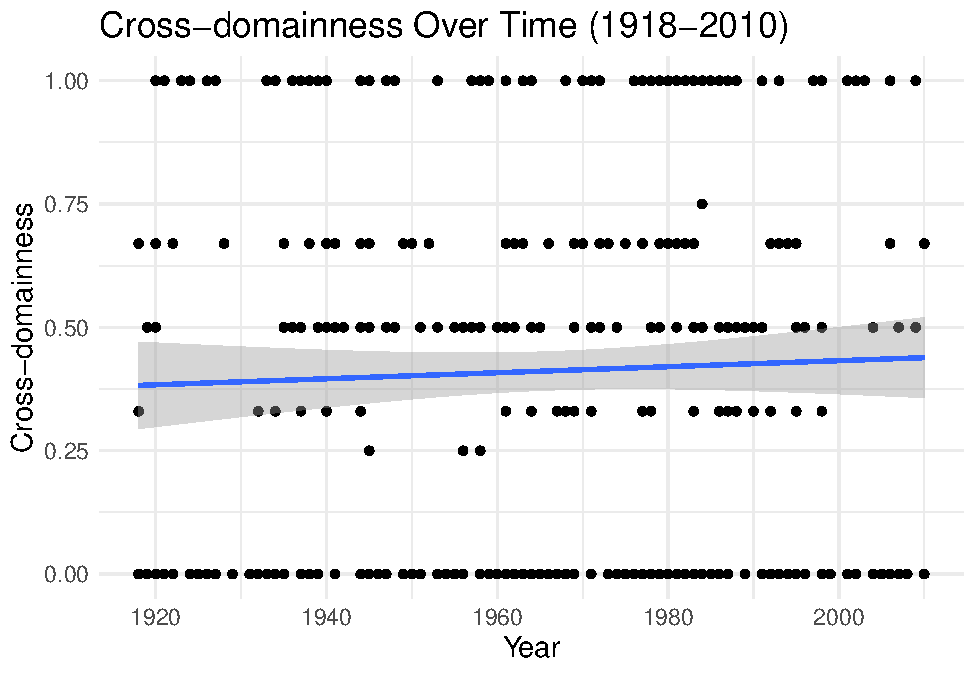
\includegraphics[width=0.8\linewidth,]{2021-03-26_ICB-Domains_files/figure-latex/cddness-time-1} 

}

\caption{Distribution of cross-domainness over time. Points represent each observation (ICB crisis) and the line represents a bivariate generalized linear model with the shaded area corresponding to the 95\% confidence interval. The slope is statistically insignificant.}\label{fig:cddness-time}
\end{figure}

\hypertarget{model}{%
\subsection{Model}\label{model}}

To test the hypotheses about the relationship between cross-domain military interactions and crisis escalation, I model the relationship using two separate independent variables --- intensity of violence and crisis duration. I choose these two dependent variables because they are common observable indicators for conflict escalation and intensity (Levy and Morgan 1984; Allen 2007; Asal and Beardsley 2007; Cederman, Warren, and Sornette 2011). The unit of analysis is the international crisis which has been collapsed down from the crisis-dyad level using the method described above.

Two different model classes are required to estimate the impact of cross-domainness on intensity of violence and crisis duration. The dependent variable for the first model --- intensity of violence --- is measured on an ordinal 1-4 scale with 1 describing no violence and 4 describing-full scale war. The dependent variable for the second model is crisis duration measured in days. Figure \ref{fig:dv} shows the distribution of the dependent variables, both of which come from the original ICB crisis-level data. The median crisis duration is 84 days. Because Model 1 has an ordinal dependent variable, the appropriate model specification is an ordered probit (Johnston, McDonald, and Quist 2020). Because Model 2 is a duration variable operationalized as the days from crisis initiation to crisis termination, I estimate a time accelerated hazard model with a log-normal parametric specification (Box-Steffensmeier and Zorn 2001; Box-Steffensmeier and Jones 2004). Time accelerated hazard models have been used to estimate factors associated with the duration of interstate or intrastate conflict by Slantchev (2004), Martinez Machain (2015), Caverley and Sechser (2017), and Chiba and Johnson (2019), among others. Although other scholars have estimated a Cox proportional hazard model (Allen 2007; Beardsley and Asal 2009; Fortna 2015), the Schoenfeld residuals for my model show that it fails the proportional hazard assumption test and is thus inappropriate here (Box-Steffensmeier, Reiter, and Zorn 2003).\footnote{Schoenfeld residuals from the proportional hazard assumption test are provided in the Online Appendix. Other parametric specifications for the hazard model are also estimated. The log-normal is used because it has the smallest AIC.}

\begin{figure}[h!]

{\centering 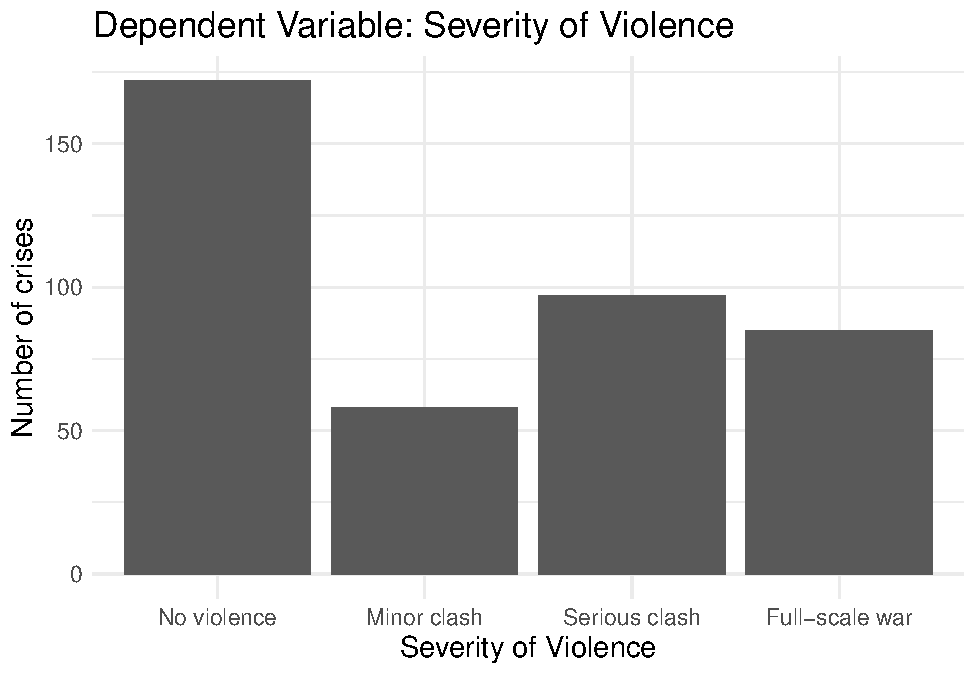
\includegraphics[width=0.8\linewidth,]{2021-03-26_ICB-Domains_files/figure-latex/dv-1} 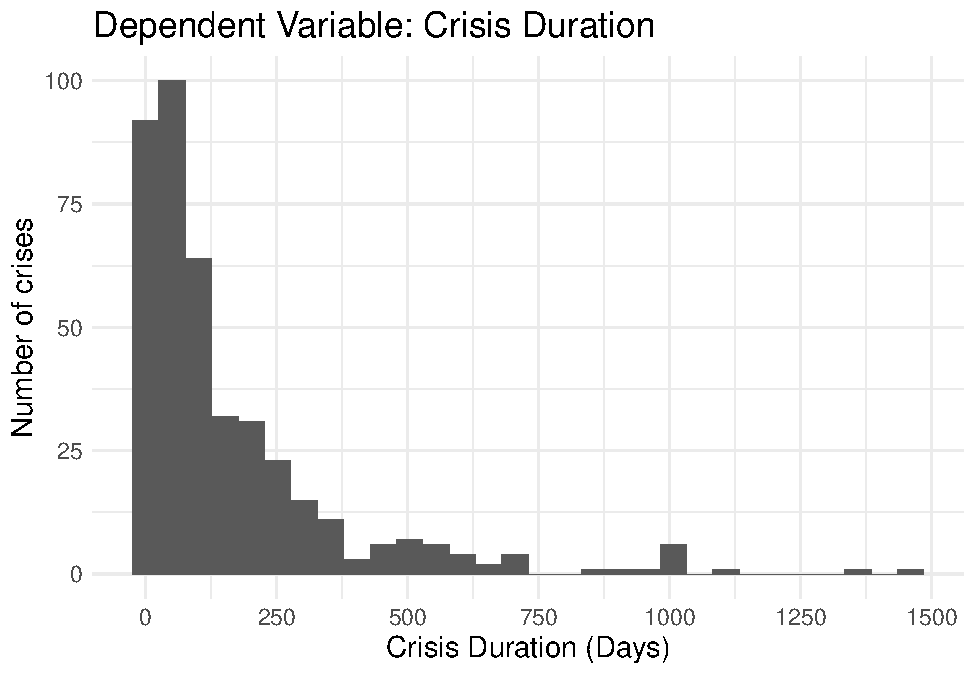
\includegraphics[width=0.8\linewidth,]{2021-03-26_ICB-Domains_files/figure-latex/dv-2} 

}

\caption{Distribution of dependent variables}\label{fig:dv}
\end{figure}

One challenge in using the crisis as the unit of analysis is that many conventional control variables that exist at the actor or sub-state level cannot be appropriately measured given difficulty in theoretically motivating the appropriate aggregation of those measures to the crisis-level (Petersen, Vasquez, and Wang 2004, 91).\footnote{This includes state-level variables like regime type and dyad-level variables like rivalry. There is a vast and well-developed literature on micro-foundations associated with the intensity and duration of conflict like leader traits and psychology. See, among others, McDermott (2004), Saunders (2009), Chiozza and Goemans (2011), Horowitz and Stam (2014), Yarhi-Milo, Lanoszka, and Cooper (2016), Renshon, Lee, and Tingley (2017), Stein (2017), and Yarhi-Milo (2018). I bracket discussion of the relationship between individual attributes and the choice of military domains for future research.} Nonetheless, both models include a battery of theoretically grounded control variables that influence the intensity and duration of international crises. I include a control for the number of crisis actors; more participants in an international crisis may make it more difficult to bargain peacefully, thus increasing the intensity and duration of a crisis (Petersen, Vasquez, and Wang 2004). I include a control for whether or not a crisis is part of a protracted conflict. Researchers have hypothesized that ongoing, embedded conflicts lead to more violent crises since they are part of a process that is more difficult to resolve (Azar, Jureidini, and McLaurin 1978; Brecher and Wilkenfeld 2000).\footnote{ICB defines a protracted conflict as ``an environment of ongoing disputes among adversaries, with fluctuating interaction ranging from violence to near-tranquility, multiple issues and spillover effects on all aspects of their relations, and the absence of mutually-recognized or anticipated termination (the Arab-Israeli conflict, 1947-)'' (Brecher et al. 2020).} I also include a control for whether the value that a crisis actor felt was threatened was territorial in nature since territorial conflicts like border wars are more violent and difficult to resolve (Vasquez 1995; Vasquez and Henehan 2001; Owsiak and Rider 2013). Territorial conflicts could also involve more similar capabilities by opposing belligerents since land and air forces may be most relevant in holding or taking territory. I include a control for whether the crisis was motivated by ethnic differences since ethnic conflicts have been shown to be more violent and difficult to resolve (Ben-Yehuda and Mishali-Ram 2006; Mishali-Ram 2006). I include a control for the degree of power disparities between each side of a crisis, which is a composite measure of population, GNP, major power alliances, territorial size, military capability, and alliance capability (Quinn et al. 2006). I further include a control for whether one of the two superpowers, the United States or Soviet Union, was involved in the crisis (Colaresi and Thompson 2002). Lastly, I control for contiguity which identifies whether or not the primary crisis actors share a border (Bremer 1992; Vasquez 1996).

\hypertarget{results}{%
\subsection{Results}\label{results}}

The full model results are detailed in Table \ref{tab:model}. For each dependent variable I first estimate a bivariate model containing only cross-domainness as an independent variable. I then estimate full models that include all control variables. For the first two models concerning crisis intensity, the results show that cross-domainness is negatively associated with the intensity of violence with statistical significance of at least the 0.01 standardized level. As the coefficients of ordered logistic regression are difficult to interpret, the odds ratio coefficient for the cross-domainness variable (0.66) indicates that the odds of a crisis with a serious clash or full scale war are 44\% lower than the odds of a crisis containing a minor clash or no violence if the actors use completely dissimilar means.\footnote{A complete table of the odds ratios is provided in the appendix.} These results provide evidence consistent with theories of cross-domain deterrence rather than cross-domain escalation --- crises in which opponents take military actions in dissimilar domains are less violent than those in which opponents take military actions in the same domains.

As models 3 and 4 are parametric time accelerated hazard models, the coefficients detail the likelihood of a crisis ending on a given day. Positive coefficients indicate a variable is associated with a longer crisis while negative coefficients mean the variable is associated with a shorter crisis duration. The coefficients for cross-domainness are negative, but not statistically significant at the 0.01 level once control variables are added to the model, meaning I cannot reject the null hypothesis that cross-domainness has no discernable effect on the duration of a crisis. The only statistically significant coefficients for crisis duration relate to the number of crisis actors and ethnic conflict. Both are statistically significant at the 0.01 level and positive, meaning that --- consistent with prior research --- crises with more actors and that are ethnic disputes are longer than crises with fewer actors or that involved other-than-ethnic issues.

\begin{table}[h!]
\begin{center}
\begin{tabular}{l c c c c}
\hline
 & \multicolumn{2}{c}{Violence Intensity} & \multicolumn{2}{c}{Crisis Duration} \\
\cline{2-3} \cline{4-5}
 & Model 1 & Model 2 & Model 3 & Model 4 \\
\hline
Cross-domainness    & $-0.50^{***}$ & $-0.41^{***}$ & $-0.29^{*}$  & $-0.21$      \\
                    & $(0.14)$      & $(0.15)$      & $(0.16)$     & $(0.17)$     \\
No. of actors       &               & $0.08^{***}$  &              & $0.07^{***}$ \\
                    &               & $(0.02)$      &              & $(0.02)$     \\
Power Dissimilarity &               & $-0.00$       &              & $0.00$       \\
                    &               & $(0.00)$      &              & $(0.01)$     \\
Protracted Crisis   &               & $0.29^{**}$   &              & $-0.12$      \\
                    &               & $(0.13)$      &              & $(0.15)$     \\
Territorial Crisis  &               & $0.09$        &              & $-0.02$      \\
                    &               & $(0.14)$      &              & $(0.16)$     \\
Major Power Involv. &               & $0.42^{***}$  &              & $0.07$       \\
                    &               & $(0.14)$      &              & $(0.16)$     \\
Ethnic Crisis       &               & $0.17$        &              & $0.65^{***}$ \\
                    &               & $(0.14)$      &              & $(0.16)$     \\
Contiguity          &               & $0.25^{*}$    &              & $-0.07$      \\
                    &               & $(0.15)$      &              & $(0.17)$     \\
Intercept           &               &               & $4.45^{***}$ & $3.86^{***}$ \\
                    &               &               & $(0.09)$     & $(0.23)$     \\
Log (scale)         &               &               & $0.29^{***}$ & $0.25^{***}$ \\
                    &               &               & $(0.03)$     & $(0.04)$     \\
\hline
AIC                 & $1071.81$     & $884.31$      & $4981.74$    & $4307.61$    \\
BIC                 & $1087.90$     & $926.99$      & $4993.80$    & $4346.41$    \\
Log Likelihood      & $-531.91$     & $-431.15$     & $-2487.87$   & $-2143.80$   \\
Deviance            & $1063.81$     & $862.31$      & $$           & $$           \\
Num. obs.           & $412$         & $358$         & $412$        & $358$        \\
\hline
\multicolumn{5}{l}{\scriptsize{\parbox{.75\linewidth}{\vspace{2pt}$^{***}p<0.01$; $^{**}p<0.05$; $^{*}p<0.1$. \\ 
                              Models 1 and 2 are ordered probit models and models 3 and 4 are log-normal accelerated failure time models.}}}
\end{tabular}
\caption{Statistical models}
\label{tab:model}
\end{center}
\end{table}

These findings are robust across a range of alternate modeling decisions, as detailed in the appendix. I run additional models using a binary dependent variable for violence severity, a modeling decision used in prior work on ICB crisis violence (Hewitt and Wilkenfeld 1996; Chiozza and Goemans 2004). Despite the appropriateness of ordered probit and a log-normal parametric specification for the duration model, I also find consistent results using ordered logistic and OLS regression for the severity of violence variable and using other parametric specifications for the crisis duration dependent variable.\footnote{The other parametric specifications for the duration model detailed in the appendix include Weibull, exponential, Gaussian, logistic, and log-logistic.}

Crises in which belligerents interact in dissimilar military domains are less violent, but neither longer nor shorter, than crises in which belligerents interact with like-means. While contemporary cross-domain conflicts with new modes of conflicts have ignited pessimism about the escalatory potential of new modes of conflict, the empirical evidence should give observers some confidence that they can respond to adversarial' ``apples'' with their own ``oranges'' without needing to be overly worried that this transition itself will result in a bloodier and longer contest. As this is a large-n study that relies on observational data, it is difficult to determine the causal direction of the relationships I characterize here. This paper has proposed one mechanism by which cross-domain interactions could reduce the severity and duration of a crisis. The causal arrow may of course run the other way. It could be that the more a state cares about the outcome of a crisis, the more likely they are to bring their best military assets to the fight. Doing so may cause less blood to be spilled since bringing mobility, stealth, and complexity to the battlefield signals to one's opponent that they are better off resolving the dispute without resorting to violence.

\hypertarget{implications-of-bringing-a-knife-to-a-gun-fight}{%
\section{Implications of bringing a knife to a gun fight}\label{implications-of-bringing-a-knife-to-a-gun-fight}}

Emerging interest in understanding cross-domain military interactions is well-deserved, given the frequency with which these interactions occur. But this research need not be spurred by, not limited to, the study of new domains made possible because of emerging technologies. Crises have always been cross-domain. Indeed, contrary to the convictions of many observers, this evidence seems to show that cross-domainness is both common and has not risen appreciably over almost a century. Importantly, this suggests that theories that concern interactions involving new domains of conflict need not reinvent the wheel since cross-domain interactions have themselves been a consistent regularity for the past century. At the same time, these findings point both to the need, and the ability, to better theorize cross-domain conflict. It can no longer be an excuse to claim that cross-domain conflict is too ``new'' to be understood even as its modality makes its understanding critical for a comprehensive appreciation of conflict processes more broadly. Different ways of defining and thinking about domains may produce new insights and certainly new domains should be compared to more traditional ones, but the findings here represent an important and thus far underrepresented contribution to that discussion.

Concerns about the escalation dynamic of cyber-kinetic interactions are loosely based off of theories of deterrence and spiral models of conflict that have rarely accounted for the strategic interaction of the military domains used during conflict. The common assumption held by pessimists is that cross-domain interactions risk a dangerous spiral because of potential miscommunication over proportionality, stake, and resolve. In contrast, the evidence provided here suggests that cross-domain interactions contain elements of the stability-instability paradox, where one side's willingness to operate in a new domain of conflict---a potential indicator of a willingness to escalate---creates conditions that lessen observed crisis escalation. This paper builds on the state of the art by furthering our understanding of conflict escalation. At least one part of the story in explaining why some conflicts spiral while others deter concerns the interaction between the domains in which each side's military is taking action. These insights help us answer the question about whether emerging technologies will make conflicts worse or whether they will prove stabilizing (Sechser, Narang, and Talmadge 2019; Talmadge 2019). Attempts to use full-spectrum combined arms forces may make sense from a strategic standpoint if they increase the probability of victory --- an outcome not examined here --- but those doing so should consider preparing for a bloodier war if their opponents is not already using, or is unlikely to respond with, their own full-spectrum combined arms forces.

The escalatory effects of the tools used in a crisis are fundamental to understanding the evolution of conflict in the 21\textsuperscript{st} century. These findings have implications for a number of contemporary policy debates. Recent work has investigated how other states can best combat Chinese naval expansion (Beckley 2017; Talmadge 2019; Cunningham 2020). As the United States considers anti-access/anti-denial (A2/AD) in East Asia vis-a-vis competition with China, strategies that seek to take advantage of full-spectrum combined-arms forces where China does not, blending multiple military tools together as done with AirSea Battle, may invoke a less bloody contest than mirroring China's moves and operating in the same military domains that they do. As NATO considers how to respond to Russian gray zone aggression, whether ``little green men'' in Crimea or cyber attacks against Estonia, responding with other non-cyber or non-special operations capabilities may not be as escalatory as alarmists argued after Israel responded to Hamas cyberattacks with missile strikes. At the very least, responding to cyber attacks with actions in kinetic domains -- whether raising alert levels, military mobilizations, training exercises, or shows of force -- could present an ideal way to signal resolve and intent in a way that prompts a de-escalatory response rather than an escalatory one.

There is much more to be studied and learned about how states fight, both as an independent variable explaining other outcomes of interest and also as a dependent variable of interest itself. As the primary contribution of this paper concerns new data on domain-interactions over the past century, I hope part of its value comes in opening up many other avenues for research concerning questions this paper raises but does not answer. Not all cross-domain interactions are created equal. While the theories tested here concern general cross-domain escalation dynamics, a land vs air conflict may turn out differently than a land vs sea conflict, although both are quantitatively measured as identically ``cross-domain''. There are specific contexts where that may be especially true, like the Indian subcontinent, where Pakistani concerns about Indian mobilization of integrated battle groups may shift the cross-domain dynamic in ways not explained here (Ganguly and Kapur 2010, 76--78). Future work should also examine the sequence of when actors take actions in different domains, since that matters for theories of first-mover advantage and unintended escalation (Quester 1977; Reiter 2009; Garfinkel and Dafoe 2019). Furthermore, the data as presented here makes simplifying aggregations regarding the domains in which states take actions during international crises. Future work can disaggregate each of those. By looking at military units instead of domains, theories can be further refined since, for example, not all naval capabilities are the same in terms of things like signaling or warfighting (Handberg 2016; Redford 2019; Gartzke and Lindsay 2020). ``Actions'' can also be further disaggregated, as further work with the underlying data could parse out and evaluate differences between things like mobilizations, raises in alert level, bombardments, and occupations as well as evaluating non-actions like speeches and cognitions. The theory and findings here are also limited to military domains, but the interaction between a state's use of military, economic, and diplomatic tools would also contribute to our collective understanding of crisis escalation and duration. Lastly, this paper investigates military domains as an independent variable in the hopes of furthering our understanding of how the choice of military domains is associated with crisis intensity and duration. I have not explained why states choose to operate in some military domains as opposed to others. Future work should think of the military domains or crisis behavior as a dependent variable and use this novel data to explain why states choose the operate in the domains that they do.

\hypertarget{conclusion}{%
\section{Conclusion}\label{conclusion}}

Much more needs to be done to better understand why nations invest, operate, and compete in particular domains. Often, they choose to fight in some domains and not others, despite the ability to do so. Why do some nations build big navies while others rely more heavily on land or air power? Does cyber (or space) offer significant advantages to challengers or to status quo actors? When does it make sense to pursue multi-domain conflict and when are nations better off limiting the horizontal spread of their uses of force? All of these questions require additional assessment, but begin to be within empirical reach, given the data I have presented and utilized here.

Epidemiologists spend much of their time identifying factors that increase the risk of particular health problems in individuals. An important component of their work relies on the proper identification of events and conditions that serve as an indicator that health problems will soon follow. Similarly, scholars of international relations are interested in identifying factors that indicate that the outbreak of conflict is increasingly likely (Senese and Vasquez 2008). The goal in this case is not only to causally identify factors that make war more likely so that we can better understand events of the past, but also to improve our ability to forecast the likelihood of conflict in the future (Valeriano and Marin 2010). The military domains in which states contest one another and the characteristics of those domains constitutes an important piece of that puzzle. Cross-domain contests in which states engage each other with dissimilar military means are less violent and endure no longer than crises in which states respond to each other in-kind. There may be other reasons to sound the alarm over emerging technologies, but the historical record shows that responding to aggression in a new and unfamiliar domain in itself does not constitute a higher risk of conflict. Contrary to the rising sense of concern among policy practitioners and military experts, cross-domain interactions are more often associate with deterring conflict than inflaming it.

\hypertarget{references}{%
\section*{References}\label{references}}
\addcontentsline{toc}{section}{References}

\hypertarget{refs}{}
\leavevmode\hypertarget{ref-ahlgren_requirementscocitationsimilarity_2003}{}%
Ahlgren, Per, Bo Jarneving, and Ronald Rousseau. 2003. ``Requirements for a Cocitation Similarity Measure, with Special Reference to Pearson's Correlation Coefficient.'' \emph{Journal of the American Society for Information Science and Technology} 54 (6): 550--60. \url{https://doi.org/10.1002/asi.10242}.

\leavevmode\hypertarget{ref-allen_timebombsestimating_2007}{}%
Allen, Susan Hannah. 2007. ``Time Bombs: Estimating the Duration of Coercive Bombing Campaigns.'' \emph{Journal of Conflict Resolution} 51 (1): 112--33. \url{https://doi.org/10.1177/0022002706296153}.

\leavevmode\hypertarget{ref-allen_understandingimpactair_2017}{}%
Allen, Susan Hannah, and Carla Martinez Machain. 2017. ``Understanding the Impact of Air Power.'' \emph{Conflict Management and Peace Science} 36 (5): 545--58. \url{https://doi.org/10.1177/0738894216682485}.

\leavevmode\hypertarget{ref-allison_armamentsarmscontrol_1975}{}%
Allison, Graham T., and Frederic A. Morris. 1975. ``Armaments and Arms Control: Exploring the Determinants of Military Weapons.'' \emph{Daedalus} 104 (3): 99--129.

\leavevmode\hypertarget{ref-althaus_clinecenterhistorical_2020}{}%
Althaus, Scott, Joseph Bajjalieh, John Carter, Buddy Peyton, and Dan Shalmon. 2020. ``Cline Center Historical Phoenix Event Data.'' University of Illinois at Urbana-Champaign: Cline Center for Advanced Social Research.

\leavevmode\hypertarget{ref-altman_advancingattackingstrategic_2018}{}%
Altman, Dan. 2018. ``Advancing Without Attacking: The Strategic Game Around the Use of Force.'' \emph{Security Studies} 27 (1): 58--88. \url{https://doi.org/10.1080/09636412.2017.1360074}.

\leavevmode\hypertarget{ref-asal_proliferationinternationalcrisis_2007}{}%
Asal, Victor, and Kyle Beardsley. 2007. ``Proliferation and International Crisis Behavior.'' \emph{Journal of Peace Research} 44 (2): 139--55. \url{https://doi.org/10.1177/0022343307075118}.

\leavevmode\hypertarget{ref-azar_protractedsocialconflict_1978}{}%
Azar, Edward E., Paul Jureidini, and Ronald McLaurin. 1978. ``Protracted Social Conflict; Theory and Practice in the Middle East.'' \emph{Journal of Palestine Studies} 8 (1): 41--60. \url{https://doi.org/10.2307/2536101}.

\leavevmode\hypertarget{ref-beardsley_winningbomb_2009}{}%
Beardsley, Kyle, and Victor Asal. 2009. ``Winning with the Bomb.'' \emph{Journal of Conflict Resolution} 53 (2): 278--301. \url{https://doi.org/10.1177/0022002708330386}.

\leavevmode\hypertarget{ref-beasley_closingpresencegap_2015}{}%
Beasley, William M. 2015. ``Closing the Presence GAP.'' \emph{Proceedings} 141 (11): 52--58.

\leavevmode\hypertarget{ref-becker_clearingairtransatlantic_2017}{}%
Becker, Jordan. 2017. ``Clearing the Air on Transatlantic Burden-Sharing, Part 2: You Gotta Give (Inputs) to Get (Outputs).'' \emph{War on the Rocks}. https://warontherocks.com/2017/05/clearing-the-air-on-transatlantic-burden-sharing-part-2-you-gotta-give-inputs-to-get-outputs/.

\leavevmode\hypertarget{ref-beckley_emergingmilitarybalance_2017}{}%
Beckley, Michael. 2017. ``The Emerging Military Balance in East Asia: How China's Neighbors Can Check Chinese Naval Expansion.'' \emph{International Security} 42 (2): 78--119. \url{https://doi.org/10.1162/ISEC_a_00294}.

\leavevmode\hypertarget{ref-ben-yehuda_ethnicactorsinternational_2006}{}%
Ben-Yehuda, Hemda, and Meirav Mishali-Ram. 2006. ``Ethnic Actors and International Crises: Theory and Findings, 19182001.'' \emph{International Interactions} 32 (1): 49--78. \url{https://doi.org/10.1080/03050620600584435}.

\leavevmode\hypertarget{ref-biddle_militarypowerexplaining_2005}{}%
Biddle, Stephen. 2005. \emph{Military Power: Explaining Victory and Defeat in Modern Battle}. Manas Publications.

\leavevmode\hypertarget{ref-biddle_strategywar_2007}{}%
---------. 2007. ``Strategy in War.'' \emph{PS: Political Science \& Politics} 40 (3): 461--66. \url{https://doi.org/10.1017/S1049096507070941}.

\leavevmode\hypertarget{ref-biddle_futurewarfarewestern_2016}{}%
Biddle, Stephen, and Ivan Oelrich. 2016. ``Future Warfare in the Western Pacific: Chinese Antiaccess/Area Denial, U.S. AirSea Battle, and Command of the Commons in East Asia.'' \emph{International Security} 41 (1): 7--48. \url{https://doi.org/10.1162/ISEC_a_00249}.

\leavevmode\hypertarget{ref-boot_warmadenew_2006}{}%
Boot, Max. 2006. \emph{War Made New: Weapons, Warriors, and the Making of the Modern World}. Penguin.

\leavevmode\hypertarget{ref-borghard_israelrespondedhamas_2019}{}%
Borghard, Erica D., and Jacquelyn Schneider. 2019. ``Israel Responded to a Hamas Cyberattack with an Airstrike. That's Not Such a Big Deal.'' \emph{Washington Post}, May.

\leavevmode\hypertarget{ref-borghard_logiccoercioncyberspace_2017}{}%
Borghard, Erica, and Shawn Lonergan. 2017. ``The Logic of Coercion in Cyberspace.'' \emph{Security Studies} 26 (3): 452--81. \url{https://doi.org/10.1080/09636412.2017.1306396}.

\leavevmode\hypertarget{ref-box-steffensmeier_eventhistorymodeling_2004}{}%
Box-Steffensmeier, Janet M., and Bradford S. Jones. 2004. \emph{Event History Modeling: A Guide for Social Scientists}. Cambridge University Press.

\leavevmode\hypertarget{ref-box-steffensmeier_nonproportionalhazardsevent_2003}{}%
Box-Steffensmeier, Janet M., Dan Reiter, and Christopher Zorn. 2003. ``Nonproportional Hazards and Event History Analysis in International Relations.'' \emph{Journal of Conflict Resolution} 47 (1): 33--53. \url{https://doi.org/10.1177/0022002702239510}.

\leavevmode\hypertarget{ref-box-steffensmeier_durationmodelsproportional_2001}{}%
Box-Steffensmeier, Janet M., and Christopher J. W. Zorn. 2001. ``Duration Models and Proportional Hazards in Political Science.'' \emph{American Journal of Political Science} 45 (4): 972--88. \url{https://doi.org/10.2307/2669335}.

\leavevmode\hypertarget{ref-boyle_costsconsequencesdrone_2013}{}%
Boyle, Michael J. 2013. ``The Costs and Consequences of Drone Warfare.'' \emph{International Affairs} 89 (1): 1--29. \url{https://doi.org/10.1111/1468-2346.12002}.

\leavevmode\hypertarget{ref-brands_paradoxesgrayzone_2016}{}%
Brands, Hal. 2016. ``Paradoxes of the Gray Zone.'' SSRN Scholarly Paper ID 2737593. Rochester, NY: Social Science Research Network.

\leavevmode\hypertarget{ref-brecher_studycrisis_2000}{}%
Brecher, Michael, and Jonathan Wilkenfeld. 2000. \emph{A Study of Crisis}. University of Michigan Press.

\leavevmode\hypertarget{ref-brecher_internationalcrisisbehavior_2020}{}%
Brecher, Michael, Jonathan Wilkenfeld, Kyle C. Beardsley, Patrick James, and David Quinn. 2020. ``International Crisis Behavior Data Codebook.'' Codebook Version 14.

\leavevmode\hypertarget{ref-bremer_dangerousdyadsconditions_1992}{}%
Bremer, Stuart A. 1992. ``Dangerous Dyads: Conditions Affecting the Likelihood of Interstate War, 1816-1965.'' \emph{The Journal of Conflict Resolution} 36 (2): 309--41.

\leavevmode\hypertarget{ref-burr_nixonadministrationhorror_2005}{}%
Burr, William. 2005. ``The Nixon Administration, the "Horror Strategy," and the Search for Limited Nuclear Options, 1969-1972: Prelude to the Schlesinger Doctrine.'' \emph{Journal of Cold War Studies} 7 (3): 34--78.

\leavevmode\hypertarget{ref-buzan_armsdynamicworld_1998}{}%
Buzan, Barry, and Eric Herring. 1998. \emph{The Arms Dynamic in World Politics}. Lynne Rienner Publishers.

\leavevmode\hypertarget{ref-byman_whydroneswork_2013}{}%
Byman, Daniel. 2013. ``Why Drones Work: The Case for Washington's Weapon of Choice.'' \emph{Foreign Affairs} 92 (4): 32--43.

\leavevmode\hypertarget{ref-cappellazielinski_politicaleconomynational_2016}{}%
Cappella Zielinski, Rosella. 2016. ``Political Economy of National Security.'' Edited by Patrick James. \emph{Oxford Bibliographies in International Relations}. New York, NY: Oxford University Press. \url{https://doi.org/10.1093/obo/9780199743292-0184}.

\leavevmode\hypertarget{ref-cappellazielinski_organizingperformancecoalition_2020}{}%
Cappella Zielinski, Rosella, and Ryan Grauer. 2020. ``Organizing for Performance: Coalition Effectiveness on the Battlefield.'' \emph{European Journal of International Relations} 26 (4): 953--78. \url{https://doi.org/10.1177/1354066120903369}.

\leavevmode\hypertarget{ref-carcelli_introducinginternationalcrisis_2021}{}%
Carcelli, Shannon, Rex W Douglass, J Andrés Gannon, and Thomas Leo Scherer. 2021. ``Introducing the International Crisis Behavior Event (ICBe) Dataset.'' Working Paper.

\leavevmode\hypertarget{ref-carcelli_diversificationdeterrencenew_2017}{}%
Carcelli, Shannon, and Erik A. Gartzke. 2017. ``The Diversification of Deterrence: New Data and Novel Realities.'' In \emph{Oxford Research Encyclopedia of Politics}. Oxford University Press. \url{https://doi.org/10.1093/acrefore/9780190228637.013.745}.

\leavevmode\hypertarget{ref-carnegie_spotlightharshglare_2018}{}%
Carnegie, Allison, and Austin Carson. 2018. ``The Spotlight's Harsh Glare: Rethinking Publicity and International Order.'' \emph{International Organization} 72 (3): 627--57. \url{https://doi.org/10.1017/S0020818318000176}.

\leavevmode\hypertarget{ref-carson_facingsavingface_2016}{}%
Carson, Austin. 2016. ``Facing Off and Saving Face: Covert Intervention and Escalation Management in the Korean War.'' \emph{International Organization} 70 (1): 103--31. \url{https://doi.org/10.1017/S0020818315000284}.

\leavevmode\hypertarget{ref-carson_secretwarscovert_2018}{}%
---------. 2018. \emph{Secret Wars: Covert Conflict in International Politics}. Princeton Studies in International History and Politics. Princeton, NJ: Princeton University Press.

\leavevmode\hypertarget{ref-carver_conventionalwarfarenuclear_1986}{}%
Carver, Michael. 1986. ``Conventional Warfare in the Nuclear Age.'' In \emph{Makers of Modern Strategy from Machiavelli to the Nuclear Age.}, edited by Peter Paret, Gordon Craig, and Felix Gilbert, 779--814. New Jersey: Princeton University Press.

\leavevmode\hypertarget{ref-cashman_introductioncauseswar_2007}{}%
Cashman, Greg, and Leonard C. Robinson. 2007. \emph{An Introduction to the Causes of War: Patterns of Interstate Conflict from World War I to Iraq}. Rowman \& Littlefield.

\leavevmode\hypertarget{ref-caton_domainscommonscontext_2012}{}%
Caton, J. L. 2012. ``Beyond Domains, Beyond Commons: Context and Theory of Conflict in Cyberspace.'' In \emph{2012 4th International Conference on Cyber Conflict (CYCON 2012)}, 1--11.

\leavevmode\hypertarget{ref-caverley_democraticmilitarismvoting_2014}{}%
Caverley, Jonathan D. 2014. \emph{Democratic Militarism: Voting, Wealth, and War}. Cambridge University Press.

\leavevmode\hypertarget{ref-caverley_militarytechnologyduration_2017}{}%
Caverley, Jonathan D, and Todd S Sechser. 2017. ``Military Technology and the Duration of Civil Conflict.'' \emph{International Studies Quarterly} 61 (3): 704--20. \url{https://doi.org/10.1093/isq/sqx023}.

\leavevmode\hypertarget{ref-cederman_testingclausewitznationalism_2011}{}%
Cederman, Lars-Erik, T. Camber Warren, and Didier Sornette. 2011. ``Testing Clausewitz: Nationalism, Mass Mobilization, and the Severity of War.'' \emph{International Organization} 65 (4): 605--38.

\leavevmode\hypertarget{ref-chiba_militarycoalitionscrisis_2019}{}%
Chiba, Daina, and Jesse C. Johnson. 2019. ``Military Coalitions and Crisis Duration.'' \emph{Journal of Politics} 81 (4): 1466--79.

\leavevmode\hypertarget{ref-chiozza_internationalconflicttenure_2004}{}%
Chiozza, Giacomo, and H. E. Goemans. 2004. ``International Conflict and the Tenure of Leaders: Is War Still Ex Post Inefficient?'' \emph{American Journal of Political Science} 48 (3): 604--19. \url{https://doi.org/10.1111/j.0092-5853.2004.00090.x}.

\leavevmode\hypertarget{ref-chiozza_leadersinternationalconflict_2011}{}%
---------. 2011. \emph{Leaders and International Conflict}. Cambridge University Press.

\leavevmode\hypertarget{ref-cimbala_militarypersuasiondeterrence_1994}{}%
Cimbala, Stephen J. 1994. \emph{Military Persuasion: Deterrence and Provocation in Crisis and War}. Pennsylvania State University Press.

\leavevmode\hypertarget{ref-colaresi_strategicrivalriesprotracted_2002}{}%
Colaresi, Michael P., and William Thompson. 2002. ``Strategic Rivalries, Protracted Conflict, and Crisis Escalation.'' \emph{Journal of Peace Research} 39 (3): 263--87. \url{https://doi.org/10.1177/0022343302039003002}.

\leavevmode\hypertarget{ref-corbett_principlesmaritimestrategy_1911}{}%
Corbett, Julian. 1911. \emph{Some Principles of Maritime Strategy}. Longmans, Green and Co.

\leavevmode\hypertarget{ref-crisher_navalpowerendogeneity_2017}{}%
Crisher, Brian. 2017. ``Naval Power, Endogeneity, and Long-Distance Disputes.'' \emph{Research and Politics} 4 (1): 1--6.

\leavevmode\hypertarget{ref-cunningham_maritimerungescalation_2020}{}%
Cunningham, Fiona S. 2020. ``The Maritime Rung on the Escalation Ladder: Naval Blockades in a US-China Conflict.'' \emph{Security Studies} 29 (4): 730--68. \url{https://doi.org/10.1080/09636412.2020.1811462}.

\leavevmode\hypertarget{ref-dafoe_reputationstatusmotives_2014}{}%
Dafoe, Allan, Jonathan Renshon, and Paul Huth. 2014. ``Reputation and Status as Motives for War.'' \emph{Annual Review of Political Science} 17 (1): 371--93. \url{https://doi.org/10.1146/annurev-polisci-071112-213421}.

\leavevmode\hypertarget{ref-dixon_azerbaijandronesowned_2020}{}%
Dixon, Robyn. 2020. ``Azerbaijan's Drones Owned the Battlefield in Nagorno-Karabakh and Showed Future of Warfare.'' \emph{Washington Post}, November.

\leavevmode\hypertarget{ref-duffield_evolutionnatostrategy_1991}{}%
Duffield, John S. 1991. ``The Evolution of NATO's Strategy of Flexible Response: A Reinterpretation.'' \emph{Security Studies} 1 (1): 132--56. \url{https://doi.org/10.1080/09636419109347460}.

\leavevmode\hypertarget{ref-early_exploringfinalfrontier_2014}{}%
Early, Bryan R. 2014. ``Exploring the Final Frontier: An Empirical Analysis of Global Civil Space Proliferation.'' \emph{International Studies Quarterly} 58 (1): 55--67. \url{https://doi.org/10.1111/isqu.12102}.

\leavevmode\hypertarget{ref-early_spyingspacereconnaissance_2021}{}%
Early, Bryan R., and Erik Gartzke. 2021. ``Spying from Space: Reconnaissance Satellites and Interstate Disputes.'' \emph{Journal of Conflict Resolution}, March. \url{https://doi.org/10.1177/0022002721995894}.

\leavevmode\hypertarget{ref-egghe_goodpropertiessimilarity_2010}{}%
Egghe, Leo. 2010. ``Good Properties of Similarity Measures and Their Complementarity.''

\leavevmode\hypertarget{ref-erickson_dangeroustradearms_2018}{}%
Erickson, Jennifer. 2018. \emph{Dangerous Trade: Arms Exports, Human Rights, and International Reputation}. Columbia University Press.

\leavevmode\hypertarget{ref-fearon_cooperationconflictcosts_2018}{}%
Fearon, James D. 2018. ``Cooperation, Conflict, and the Costs of Anarchy.'' \emph{International Organization} 72 (3): 523--59. \url{https://doi.org/10.1017/S0020818318000115}.

\leavevmode\hypertarget{ref-fearon_rationalistexplanationswar_1995}{}%
---------. 1995. ``Rationalist Explanations for War.'' \emph{International Organization} 49 (3): 379--414. \url{https://doi.org/10.1017/S0020818300033324}.

\leavevmode\hypertarget{ref-ferreiro_horationelsonnever_2016}{}%
Ferreiro, Larrie D. 2016. ``Horatio Nelson Never Wrote `A Ship's a Fool to Fight a Fort'; It Was Jackie Fisher Who Invented the Attribution.'' \emph{Journal of Military History} 80 (3): 855--56.

\leavevmode\hypertarget{ref-fikenscher_seekingstatusrecognition_2015}{}%
Fikenscher, Sven-Eric, Lena Jaschob, and Reinhard Wolf. 2015. ``Seeking Status Recognition Through Military Symbols: German and Indian Armament Policies Between Strategic Rationalizations and Prestige Motives.'' In \emph{Recognition in International Relations: Rethinking a Political Concept in a Global Context}, edited by Christopher Daase, Caroline Fehl, Anna Geis, and Georgios Kolliarakis, 86--103. Palgrave Studies in International Relations Series. London: Palgrave Macmillan UK. \url{https://doi.org/10.1057/9781137464729_5}.

\leavevmode\hypertarget{ref-fordham_verysharpsword_2004}{}%
Fordham, Benjamin O. 2004. ``A Very Sharp Sword: The Influence of Military Capabilities on American Decisions to Use Force.'' \emph{Journal of Conflict Resolution} 48 (5): 632--56. \url{https://doi.org/10.1177/0022002704267935}.

\leavevmode\hypertarget{ref-fortna_terroristswinrebels_2015}{}%
Fortna, Virginia Page. 2015. ``Do Terrorists Win? Rebels' Use of Terrorism and Civil War Outcomes.'' \emph{International Organization} 69 (3): 519--56. \url{https://doi.org/10.1017/S0020818315000089}.

\leavevmode\hypertarget{ref-gamberini_quantumsensingpotential_2021}{}%
Gamberini, Sarah Jacobs, and Lawrence Rubin. 2021. ``Quantum Sensing's Potential Impacts on Strategic Deterrence and Modern Warfare.'' \emph{Orbis}, March. \url{https://doi.org/10.1016/j.orbis.2021.03.012}.

\leavevmode\hypertarget{ref-ganguly_indiapakistanbomb_2010}{}%
Ganguly, Sumit, and S. Paul Kapur. 2010. \emph{India, Pakistan, and the Bomb: Debating Nuclear Stability in South Asia}. New York, NY: Columbia University Press.

\leavevmode\hypertarget{ref-gannon_shadowdeterrencewhy_2021}{}%
Gannon, J Andrés, Erik A. Gartzke, Jon R. Lindsay, and Peter Schram. 2021. ``The Shadow of Deterrence: Why Capable Actors Engage in Contests Short of War.'' Working Paper.

\leavevmode\hypertarget{ref-garfinkel_howdoesoffensedefense_2019}{}%
Garfinkel, Ben, and Allan Dafoe. 2019. ``How Does the Offense-Defense Balance Scale?'' \emph{Journal of Strategic Studies} 42 (6): 736--63. \url{https://doi.org/10.1080/01402390.2019.1631810}.

\leavevmode\hypertarget{ref-gartner_openingblackbox_1998}{}%
Gartner, Scott Sigmund. 1998. ``Opening up the Black Box of War.'' \emph{Journal of Conflict Resolution} 42 (3): 252--58. \url{https://doi.org/10.1177/0022002798042003002}.

\leavevmode\hypertarget{ref-gartzke_warerrorterm_1999}{}%
Gartzke, Erik A. 1999. ``War Is in the Error Term.'' \emph{International Organization} 53 (3): 567--87. \url{https://doi.org/10.1162/002081899550995}.

\leavevmode\hypertarget{ref-gartzke_signalingforeignpolicy_2017}{}%
Gartzke, Erik A., Shannon Carcelli, J Andrés Gannon, and Jiakun Jack Zhang. 2017. ``Signaling in Foreign Policy.'' \emph{Oxford Encyclopedia of Foreign Policy Analysis}, August.

\leavevmode\hypertarget{ref-gartzke_determinantsnuclearforce_2014}{}%
Gartzke, Erik A., Jeffrey M. Kaplow, and Rupal N. Mehta. 2014. ``The Determinants of Nuclear Force Structure.'' \emph{Journal of Conflict Resolution} 58 (3): 481--508. \url{https://doi.org/10.1177/0022002713509054}.

\leavevmode\hypertarget{ref-gartzke_influenceseapower_2020}{}%
Gartzke, Erik A., and Jon R. Lindsay. 2020. ``The Influence of Sea Power on Politics: Domain- and Platform-Specific Attributes of Material Capabilities.'' \emph{Security Studies} 29 (4): 601--36. \url{https://doi.org/10.1080/09636412.2020.1811450}.

\leavevmode\hypertarget{ref-gatopoulos_nagornokarabakhconflictushering_2020}{}%
Gatopoulos, Alex. 2020. ``The Nagorno-Karabakh Conflict Is Ushering in a New Age of Warfare.'' \emph{Al Jazeera}, October.

\leavevmode\hypertarget{ref-gavin_mythflexibleresponse_2001}{}%
Gavin, Francis J. 2001. ``The Myth of Flexible Response: United States Strategy in Europe During the 1960s.'' \emph{The International History Review} 23 (4): 847--75.

\leavevmode\hypertarget{ref-glaser_politicalconsequencesmilitary_1992}{}%
Glaser, Charles L. 1992. ``Political Consequences of Military Strategy: Expanding and Refining the Spiral and Deterrence Models.'' \emph{World Politics} 44 (4): 497--538. \url{https://doi.org/10.2307/2010486}.

\leavevmode\hypertarget{ref-gleditsch_revisedlistindependent_1999}{}%
Gleditsch, Kristian S., and Michael D. Ward. 1999. ``A Revised List of Independent States Since the Congress of Vienna.'' \emph{International Interactions} 25 (4): 393--413. \url{https://doi.org/10.1080/03050629908434958}.

\leavevmode\hypertarget{ref-green_revolutionthatfailed_2020}{}%
Green, Brendan Rittenhouse. 2020. \emph{The Revolution That Failed: Nuclear Competition, Arms Control, and the Cold War}. Cambridge: Cambridge University Press. \url{https://doi.org/10.1017/9781108779593}.

\leavevmode\hypertarget{ref-greenhill_asymmetricadvantageweaponizing_2019}{}%
Greenhill, Kelly. 2019. ``Asymmetric Advantage: Weaponizing People as Nonmilitary Instruments in Cross-Domain Coercion.'' In \emph{Cross-Domain Deterrence: Strategy in an Era of Complexity}, edited by Jon R. Lindsay and Erik A. Gartzke, 1st edition, 259--89. New York, NY: Oxford University Press.

\leavevmode\hypertarget{ref-grimmer_machinelearningsocial_2021}{}%
Grimmer, Justin, Margaret E. Roberts, and Brandon M. Stewart. 2021. ``Machine Learning for Social Science: An Agnostic Approach.'' \emph{Annual Review of Political Science} 24 (1). \url{https://doi.org/10.1146/annurev-polisci-053119-015921}.

\leavevmode\hypertarget{ref-handberg_aircraftcarrierballistic_2016}{}%
Handberg, Roger. 2016. ``Aircraft Carrier or Ballistic Missile Defense: Signaling Commitment in Situations of Uncertainty.'' \emph{Comparative Strategy} 35 (5): 355--62. \url{https://doi.org/10.1080/01495933.2016.1240975}.

\leavevmode\hypertarget{ref-hazelton_dronestrikesgrand_2016}{}%
Hazelton, Jacqueline. 2016. ``Drone Strikes and Grand Strategy: Toward a Political Understanding of the Uses of Unmanned Aerial Vehicle Attacks in US Security Policy.'' \emph{Journal of Strategic Studies} 40 (1-2): 68--91. \url{https://doi.org/10.1080/01402390.2016.1196589}.

\leavevmode\hypertarget{ref-healey_notcyberdeterrence_2018}{}%
Healey, Jason. 2018. ``Not the Cyber Deterrence the United States Wants.'' \emph{Council on Foreign Relations Digital and Cyberspace Policy Program}.

\leavevmode\hypertarget{ref-hewitt_dyadicprocessesinternational_2003}{}%
Hewitt, J. Joseph. 2003. ``Dyadic Processes and International Crises.'' \emph{Journal of Conflict Resolution} 47 (5): 669--92. \url{https://doi.org/10.1177/0022002703252973}.

\leavevmode\hypertarget{ref-hewitt_democraciesinternationalcrisis_1996}{}%
Hewitt, J. Joseph, and Jonathan Wilkenfeld. 1996. ``Democracies in International Crisis.'' \emph{International Interactions} 22 (2): 123--42. \url{https://doi.org/10.1080/03050629608434885}.

\leavevmode\hypertarget{ref-hicks_othermeanspart_2019}{}%
Hicks, Kathleen H., and Alice Hunt Friend. 2019. ``By Other Means Part I: Campaigning in the Gray Zone.'' Lanham: Center for Strategic \& International Studies.

\leavevmode\hypertarget{ref-horowitz_artificialintelligenceinternational_2018}{}%
Horowitz, Michael C. 2018. ``Artificial Intelligence, International Competition, and the Balance of Power.'' \emph{Texas National Security Review} 1 (3): 37--57. \url{https://doi.org/10.15781/T2639KP49}.

\leavevmode\hypertarget{ref-horowitz_emergingmilitarytechnologies_2020}{}%
---------. 2020. ``Do Emerging Military Technologies Matter for International Politics?'' \emph{Annual Review of Political Science} 23 (1): 385--400. \url{https://doi.org/10.1146/annurev-polisci-050718-032725}.

\leavevmode\hypertarget{ref-horowitz_diffusionmilitarypower_2010}{}%
---------. 2010. \emph{The Diffusion of Military Power: Causes and Consequences for International Politics}. Princeton University Press.

\leavevmode\hypertarget{ref-horowitz_consequencesdroneproliferation_2016}{}%
Horowitz, Michael C., Sarah E. Kreps, and Matthew Fuhrmann. 2016. ``The Consequences of Drone Proliferation: Separating Fact from Fiction.'' \emph{International Security} 41 (2): 7--42.

\leavevmode\hypertarget{ref-horowitz_howpriormilitary_2014}{}%
Horowitz, Michael C., and Allan C. Stam. 2014. ``How Prior Military Experience Influences the Future Militarized Behavior of Leaders.'' \emph{International Organization} 68 (03): 527--59. \url{https://doi.org/10.1017/S0020818314000046}.

\leavevmode\hypertarget{ref-huang_militarydeterrencemultidimensionality_2019}{}%
Huang, Chin-Hao, and David Kang. 2019. ``Beyond Military Deterrence: The Multidimensionality of International Relations in East Asia.'' In \emph{Cross-Domain Deterrence: Strategy in an Era of Complexity}, edited by Jon R. Lindsay and Erik A. Gartzke, 1st edition, 317--34. New York, NY: Oxford University Press.

\leavevmode\hypertarget{ref-jensen_algorithmswarpromise_2020}{}%
Jensen, Benjamin M, Christopher Whyte, and Scott Cuomo. 2020. ``Algorithms at War: The Promise, Peril, and Limits of Artificial Intelligence.'' \emph{International Studies Review} 22 (3): 526--50. \url{https://doi.org/10.1093/isr/viz025}.

\leavevmode\hypertarget{ref-jervis_illogicamericannuclear_1984}{}%
Jervis, Robert. 1984. \emph{The Illogic of American Nuclear Strategy}. Cornell University Press.

\leavevmode\hypertarget{ref-johnson_delegatingstrategicdecisionmaking_2020}{}%
Johnson, James. 2020. ``Delegating Strategic Decision-Making to Machines: Dr. Strangelove Redux?'' \emph{Journal of Strategic Studies} 0 (0): 1--39. \url{https://doi.org/10.1080/01402390.2020.1759038}.

\leavevmode\hypertarget{ref-johnston_generalizedorderedprobit_2020}{}%
Johnston, Carla, James McDonald, and Kramer Quist. 2020. ``A Generalized Ordered Probit Model.'' \emph{Communications in Statistics - Theory and Methods} 49 (7): 1712--29. \url{https://doi.org/10.1080/03610926.2019.1565780}.

\leavevmode\hypertarget{ref-kahn_thermonuclearwar_2007}{}%
Kahn, Herman. 2007. \emph{On Thermonuclear War}. New Brunswick {[}N.J.: Transaction Publishers.

\leavevmode\hypertarget{ref-kahn_whogetssmart_2021}{}%
Kahn, Lauren, and Michael C. Horowitz. 2021. ``Who Gets Smart: Explaining How Precision Bombs Proliferate.'' SSRN Scholarly Paper ID 3792071. Rochester, NY: Social Science Research Network. \url{https://doi.org/10.2139/ssrn.3792071}.

\leavevmode\hypertarget{ref-kennedy_risefallbritish_1976}{}%
Kennedy, Paul M. 1976. \emph{The Rise and Fall of British Naval Mastery}. Humanity Books.

\leavevmode\hypertarget{ref-kissinger_limitedwarconventional_1960}{}%
Kissinger, Henry. 1960. ``Limited War: Conventional or Nuclear? A Reappraisal.'' \emph{Daedalus} 89 (4): 800--817.

\leavevmode\hypertarget{ref-kostyuk_invisibledigitalfront_2019}{}%
Kostyuk, Nadiya, and Yuri Zhukov. 2019. ``Invisible Digital Front: Can Cyber Attacks Shape Battlefield Events?'' \emph{Journal of Conflict Resolution} 63 (2): 317--47. \url{https://doi.org/10.1177/0022002717737138}.

\leavevmode\hypertarget{ref-kreps_escalationfirebreakscyber_2019}{}%
Kreps, Sarah, and Jacquelyn Schneider. 2019. ``Escalation Firebreaks in the Cyber, Conventional, and Nuclear Domains: Moving Beyond Effects-Based Logics.'' \emph{Journal of Cybersecurity} 5 (1): 1--11. \url{https://doi.org/10.1093/cybsec/tyz007}.

\leavevmode\hypertarget{ref-kroenig_logicamericannuclear_2018}{}%
Kroenig, Matthew. 2018. \emph{The Logic of American Nuclear Strategy: Why Strategic Superiority Matters}. Oxford University Press.

\leavevmode\hypertarget{ref-lai_effectsdifferenttypes_2004}{}%
Lai, Brian. 2004. ``The Effects of Different Types of Military Mobilization on the Outcome of International Crises.'' \emph{The Journal of Conflict Resolution} 48 (2): 211--29.

\leavevmode\hypertarget{ref-lebow_whynationsfight_2010}{}%
Lebow, Richard Ned. 2010. \emph{Why Nations Fight: Past and Future Motives for War}. Cambridge University Press.

\leavevmode\hypertarget{ref-levin-banchik_precrisismilitaryhostility_2020}{}%
Levin-Banchik, Luba. 2020. ``Precrisis Military Hostility and Escalation in International Crises.'' \emph{Conflict Management and Peace Science} 38 (1): 63--86. \url{https://doi.org/10.1177/0738894220906376}.

\leavevmode\hypertarget{ref-levy_frequencyseriousnesswar_1984}{}%
Levy, Jack S., and T. Clifton Morgan. 1984. ``The Frequency and Seriousness of War: An Inverse Relationship?'' \emph{Journal of Conflict Resolution} 28 (4): 731--49. \url{https://doi.org/10.1177/0022002784028004007}.

\leavevmode\hypertarget{ref-libicki_cyberdeterrencecyberwar_2009}{}%
Libicki, Martin C. 2009. \emph{Cyberdeterrence and Cyberwar}. Santa Monica, CA: RAND.

\leavevmode\hypertarget{ref-libicki_cyberspacenotwarfighting_2012}{}%
---------. 2012. ``Cyberspace Is Not a Warfighting Domain.'' \emph{I/S: A Journal of Law and Policy for the Information Society} 8: 321.

\leavevmode\hypertarget{ref-lieber_mythnuclearrevolution_2020}{}%
Lieber, Keir A., and Daryl G. Press. 2020. \emph{The Myth of the Nuclear Revolution: Power Politics in the Atomic Age}. Ithaca New York: Cornell University Press.

\leavevmode\hypertarget{ref-lindsay_demystifyingquantumthreat_2020}{}%
Lindsay, Jon R. 2020. ``Demystifying the Quantum Threat: Infrastructure, Institutions, and Intelligence Advantage.'' \emph{Security Studies} 29 (2): 335--61. \url{https://doi.org/10.1080/09636412.2020.1722853}.

\leavevmode\hypertarget{ref-lindsay_coercioncyberspacestabilityinstability_2018}{}%
Lindsay, Jon R., and Erik A. Gartzke. 2018. ``Coercion Through Cyberspace: The Stability-Instability Paradox Revisited.'' In \emph{Coercion: The Power to Hurt in International Politics}, edited by Kelly M. Greenhill and Peter Krause. New York, NY: Oxford University Press.

\leavevmode\hypertarget{ref-lindsay_crossdomaindeterrencestrategy_2019}{}%
---------, eds. 2019a. \emph{Cross-Domain Deterrence: Strategy in an Era of Complexity}. 1st edition. New York, NY: Oxford University Press.

\leavevmode\hypertarget{ref-lindsay_introductioncrossdomaindeterrence_2019}{}%
---------. 2019b. ``Introduction: Cross-Domain Deterrence, from Practice to Theory.'' In \emph{Cross-Domain Deterrence: Strategy in an Era of Complexity}, edited by Jon R. Lindsay and Erik Gartzke, 1st edition, 1--26. New York, NY: Oxford University Press.

\leavevmode\hypertarget{ref-lindsay_politicsmanyother_2020}{}%
---------. 2020. ``Politics by Many Other Means: The Comparative Strategic Advantages of Operational Domains.'' \emph{Journal of Strategic Studies} 0 (0): 1--34. \url{https://doi.org/10.1080/01402390.2020.1768372}.

\leavevmode\hypertarget{ref-lin-greenberg_privateeyessky_2021}{}%
Lin-Greenberg, Erik, and Theo Milonopoulos. 2021. ``Private Eyes in the Sky: Emerging Technology and the Political Consequences of Eroding Government Secrecy.'' \emph{Journal of Conflict Resolution}, February. \url{https://doi.org/10.1177/0022002720987285}.

\leavevmode\hypertarget{ref-lupton_signalingresolveleaders_2018}{}%
Lupton, Danielle L. 2018. ``Signaling Resolve: Leaders, Reputations, and the Importance of Early Interactions.'' \emph{International Interactions} 44 (1): 59--87. \url{https://doi.org/10.1080/03050629.2017.1316268}.

\leavevmode\hypertarget{ref-lyall_ragemachinesexplaining_2009}{}%
Lyall, Jason, and Isaiah Wilson. 2009. ``Rage Against the Machines: Explaining Outcomes in Counterinsurgency Wars.'' \emph{International Organization} 63 (1): 67--106. \url{https://doi.org/10.1017/S0020818309090031}.

\leavevmode\hypertarget{ref-mackey_prewarmobilizationtermination_2014}{}%
Mackey, Kyle. 2014. ``Prewar Mobilization and the Termination of Interstate Wars.'' SSRN Scholarly Paper ID 2385749. Rochester, NY: Social Science Research Network.

\leavevmode\hypertarget{ref-martinezmachain_aircampaignduration_2015}{}%
Martinez Machain, Carla. 2015. ``Air Campaign Duration and the Interaction of Air and Ground Forces.'' \emph{International Interactions} 41 (3): 539--64. \url{https://doi.org/10.1080/03050629.2015.1018414}.

\leavevmode\hypertarget{ref-mcdermott_prospecttheorypolitical_2004}{}%
McDermott, Rose. 2004. ``Prospect Theory in Political Science: Gains and Losses from the First Decade.'' \emph{Political Psychology} 25 (2): 289--312. \url{https://doi.org/10.1111/j.1467-9221.2004.00372.x}.

\leavevmode\hypertarget{ref-mcmaster_harbingersfuturewar_2016}{}%
McMaster, H. R. 2016. ``Harbingers of Future War: Implications for the Army with Lieutenant General H.R. McMaster.'' Washington, DC.

\leavevmode\hypertarget{ref-mishali-ram_ethnicdiversityissues_2006}{}%
Mishali-Ram, Meirav. 2006. ``Ethnic Diversity, Issues, and International Crisis Dynamics, 1918-2002.'' \emph{Journal of Peace Research} 43 (5): 583--600. \url{https://doi.org/10.1177/0022343306066524}.

\leavevmode\hypertarget{ref-montgomery_signalsstrengthcapability_2020}{}%
Montgomery, Evan Braden. 2020. ``Signals of Strength: Capability Demonstrations and Perceptions of Military Power.'' \emph{Journal of Strategic Studies} 43 (2): 309--30. \url{https://doi.org/10.1080/01402390.2019.1626724}.

\leavevmode\hypertarget{ref-morgan_issuelinkagesinternational_1990}{}%
Morgan, T. Clifton. 1990. ``Issue Linkages in International Crisis Bargaining.'' \emph{American Journal of Political Science} 34 (2): 311--33. \url{https://doi.org/10.2307/2111449}.

\leavevmode\hypertarget{ref-morgan_untyingknotwar_1994}{}%
---------. 1994. \emph{Untying the Knot of War: A Bargaining Theory of International Crises}. Ann Arbor: University of Michigan Press.

\leavevmode\hypertarget{ref-morgan_modelforeignpolicy_2000}{}%
Morgan, T. Clifton, and Glenn Palmer. 2000. ``A Model of Foreign Policy Substitutability: Selecting the Right Tools for the Job(s).'' \emph{Journal of Conflict Resolution} 44 (1): 11--32. \url{https://doi.org/10.1177/0022002700044001002}.

\leavevmode\hypertarget{ref-morris_israelgazamilitants_2019}{}%
Morris, Loveday, Ruth Eglash, and Hazem Balousha. 2019. ``Israel and Gaza Militants Agree to Cease-Fire After Weekend of Violence.'' \emph{Washington Post}, May.

\leavevmode\hypertarget{ref-morrow_internationallawcommon_2019}{}%
Morrow, James. 2019. ``International Law and the Common Knowledge Requirements of Cross-Domain Deterrence.'' In \emph{Cross-Domain Deterrence: Strategy in an Era of Complexity}, edited by Jon R. Lindsay and Erik A. Gartzke, 1st edition, 187--204. New York, NY: Oxford University Press.

\leavevmode\hypertarget{ref-newman_whatisraelstrike_2019}{}%
Newman, Lily Hay. 2019. ``What Israel's Strike on Hamas Hackers Means for Cyberwar.'' \emph{Wired}, May.

\leavevmode\hypertarget{ref-nye_deterrencedissuasioncyberspace_2017}{}%
Nye, Joseph. 2017. ``Deterrence and Dissuasion in Cyberspace.'' \emph{International Security} 41 (3): 44--71. \url{https://doi.org/10.1162/ISEC_a_00266}.

\leavevmode\hypertarget{ref-oneill_conflictualmovesbargaining_1991}{}%
O'Neill, Barry. 1991. ``Conflictual Moves in Bargaining: Warnings, Threats, Escalations, and Ultimatums.'' In \emph{Negotiation Analysis}, edited by H. Peyton Young, 87--108. University of Michigan Press.

\leavevmode\hypertarget{ref-owsiak_clearinghurdleborder_2013}{}%
Owsiak, Andrew P., and Toby J. Rider. 2013. ``Clearing the Hurdle: Border Settlement and Rivalry Termination.'' \emph{The Journal of Politics} 75 (3): 757--72. \url{https://doi.org/10.1017/S0022381613000595}.

\leavevmode\hypertarget{ref-paul_statusworldpolitics_2014}{}%
Paul, T. V., Deborah Welch Larson, and William C. Wohlforth. 2014. \emph{Status in World Politics}. Cambridge University Press.

\leavevmode\hypertarget{ref-petersen_multipartydisputesprobability_2004}{}%
Petersen, Karen K., John A. Vasquez, and Yijia Wang. 2004. ``Multiparty Disputes and the Probability of War, 18161992.'' \emph{Conflict Management and Peace Science} 21 (2): 85--100. \url{https://doi.org/10.1080/07388940490463898}.

\leavevmode\hypertarget{ref-poast_doesissuelinkage_2012}{}%
Poast, Paul. 2012. ``Does Issue Linkage Work? Evidence from European Alliance Negotiations, 1860 to 1945.'' \emph{International Organization} 66 (2): 277--310. \url{https://doi.org/10.1017/S0020818312000069}.

\leavevmode\hypertarget{ref-post_flyingfailcostly_2019}{}%
Post, Abigail. 2019. ``Flying to Fail: Costly Signals and Air Power in Crisis Bargaining.'' \emph{Journal of Conflict Resolution} 63 (4): 869--95. \url{https://doi.org/10.1177/0022002718777043}.

\leavevmode\hypertarget{ref-powell_stabilitydistributionpower_1996}{}%
Powell, Robert. 1996. ``Stability and the Distribution of Power.'' \emph{World Politics} 48 (2): 239--67. \url{https://doi.org/10.1353/wp.1996.0006}.

\leavevmode\hypertarget{ref-powell_nuclearbrinkmanshiplimited_2015}{}%
---------. 2015. ``Nuclear Brinkmanship, Limited War, and Military Power.'' \emph{International Organization} 69 (3): 589--626. \url{https://doi.org/10.1017/S0020818315000028}.

\leavevmode\hypertarget{ref-quek_arecostlysignals_2013}{}%
Quek, Kai. 2013. ``Are Costly Signals More Credible? Evidence from Three Experiments.'' \emph{SSRN Electronic Journal}. \url{https://doi.org/10.2139/ssrn.2256528}.

\leavevmode\hypertarget{ref-quester_offensedefenseinternational_1977}{}%
Quester, George H. 1977. \emph{Offense and Defense in the International System}. Transaction Books.

\leavevmode\hypertarget{ref-quinn_powerplaymediation_2006}{}%
Quinn, David, Jonathan Wilkenfeld, Kathleen Smarick, and Victor Asal. 2006. ``Power Play: Mediation in Symmetric and Asymmetric International Crises.'' \emph{International Interactions} 32 (4): 441--70. \url{https://doi.org/10.1080/03050620601011107}.

\leavevmode\hypertarget{ref-redford_fullspectrumantisubmarine_2019}{}%
Redford, Duncan. 2019. ``Full Spectrum Anti-Submarine Warfare the Historical Evidence from a British Perspective.'' \emph{Journal of Strategic Studies} 0 (0): 1--31. \url{https://doi.org/10.1080/01402390.2019.1623029}.

\leavevmode\hypertarget{ref-reiter_howwarsend_2009}{}%
Reiter, Dan. 2009. \emph{How Wars End}. Princeton University Press.

\leavevmode\hypertarget{ref-renshon_statusdeficitswar_2016}{}%
Renshon, Jonathan. 2016. ``Status Deficits and War.'' \emph{International Organization} 70 (03): 513--50. \url{https://doi.org/10.1017/S0020818316000163}.

\leavevmode\hypertarget{ref-renshon_emotionsmicrofoundationscommitment_2017}{}%
Renshon, Jonathan, Julia J. Lee, and Dustin Tingley. 2017. ``Emotions and the Micro-Foundations of Commitment Problems.'' \emph{International Organization} 71 (S1): S189--S218. \url{https://doi.org/10.1017/S0020818316000473}.

\leavevmode\hypertarget{ref-rosen_winningnextwar_1991}{}%
Rosen, Stephen Peter. 1991. \emph{Winning the Next War: Innovation and the Modern Military}. Cornell University Press.

\leavevmode\hypertarget{ref-rosenau_comparativeforeignpolicy_1968}{}%
Rosenau, James N. 1968. ``Comparative Foreign Policy: Fad, Fantasy, or Field?'' \emph{International Studies Quarterly} 12 (3): 296--329. \url{https://doi.org/10.2307/3013508}.

\leavevmode\hypertarget{ref-rovner_giveinstabilitychance_2020}{}%
Rovner, Joshua. 2020. ``Give Instability a Chance?'' \emph{War on the Rocks}. https://warontherocks.com/2020/07/give-instability-a-chance/.

\leavevmode\hypertarget{ref-sagan_madmannuclearalert_2003}{}%
Sagan, Scott Douglas, and Jeremi Suri. 2003. ``The Madman Nuclear Alert: Secrecy, Signaling, and Safety in October 1969.'' \emph{International Security} 27 (4): 150--83.

\leavevmode\hypertarget{ref-sanger_chinaappearswarn_2021}{}%
Sanger, David E., and Emily Schmall. 2021. ``China Appears to Warn India: Push Too Hard and the Lights Could Go Out.'' \emph{The New York Times}, February.

\leavevmode\hypertarget{ref-saunders_transformativechoicesleaders_2009}{}%
Saunders, Elizabeth N. 2009. ``Transformative Choices: Leaders and the Origins of Intervention Strategy.'' \emph{International Security} 34 (2): 119--61. \url{https://doi.org/10.1162/isec.2009.34.2.119}.

\leavevmode\hypertarget{ref-schilde_europeanmilitarycapabilities_2017}{}%
Schilde, Kaija. 2017. ``European Military Capabilities: Enablers and Constraints on EU Power?'' \emph{JCMS: Journal of Common Market Studies} 55 (1): 37--53. \url{https://doi.org/10.1111/jcms.12444}.

\leavevmode\hypertarget{ref-schneider_informationrevolutioninternational_2017}{}%
Schneider, Jacquelyn. 2017. ``The Information Revolution and International Stability: A Multi-Article Exploration of Computing, Cyber, and Incentives for Conflict.'' Dissertation, Washington, D.C.: George Washington University.

\leavevmode\hypertarget{ref-schneider_whytroopsdon_2017}{}%
Schneider, Jacquelyn, and Julia M. Macdonald. 2017. ``Why Troops Don't Trust Drones.'' \emph{Foreign Affairs}, December.

\leavevmode\hypertarget{ref-schrodt_precedentsprogressprospects_2012}{}%
Schrodt, Philip A. 2012. ``Precedents, Progress, and Prospects in Political Event Data.'' \emph{International Interactions} 38 (4): 546--69. \url{https://doi.org/10.1080/03050629.2012.697430}.

\leavevmode\hypertarget{ref-schrodt_cameoconflictmediation_2005}{}%
Schrodt, Philip A., Deborah Gerner, Ömur Yilmaz, and Dennis Hermreck. 2005. ``The CAMEO (Conflict and Mediation Event Observations) Actor Coding Framework.'' In \emph{American Political Science Association Annual Meeting}. Washington, DC.

\leavevmode\hypertarget{ref-sechser_emergingtechnologiesstrategic_2019}{}%
Sechser, Todd S., Neil Narang, and Caitlin Talmadge. 2019. ``Emerging Technologies and Strategic Stability in Peacetime, Crisis, and War.'' \emph{Journal of Strategic Studies} 42 (6): 727--35. \url{https://doi.org/10.1080/01402390.2019.1626725}.

\leavevmode\hypertarget{ref-senese_stepswarempirical_2008}{}%
Senese, Paul D., and John A. Vasquez. 2008. \emph{The Steps to War: An Empirical Study}. Princeton University Press.

\leavevmode\hypertarget{ref-shifrinson_linkagepoliticsmanaging_2019}{}%
Shifrinson, Joshua R. Itzkowitz. 2019. ``Linkage Politics: Managing the End of the Cold War.'' In \emph{Cross-Domain Deterrence: Strategy in an Era of Complexity}, edited by Jon R. Lindsay and Erik A. Gartzke, 1st edition, 290--316. New York, NY: Oxford University Press.

\leavevmode\hypertarget{ref-slantchev_powerhurtcostly_2003}{}%
Slantchev, Branislav L. 2003. ``The Power to Hurt: Costly Conflict with Completely Informed States.'' \emph{The American Political Science Review} 97 (1): 123--33. \url{https://doi.org/10.2307/3118225}.

\leavevmode\hypertarget{ref-slantchev_howinitiatorsend_2004}{}%
---------. 2004. ``How Initiators End Their Wars: The Duration of Warfare and the Terms of Peace.'' \emph{American Journal of Political Science} 48 (4): 813--29. \url{https://doi.org/10.1111/j.0092-5853.2004.00103.x}.

\leavevmode\hypertarget{ref-slantchev_militarycoercioninterstate_2005}{}%
---------. 2005. ``Military Coercion in Interstate Crises.'' \emph{American Political Science Review} 99 (4): 533--47. \url{https://doi.org/10.1017/S0003055405051865}.

\leavevmode\hypertarget{ref-slantchev_militarythreatscosts_2011}{}%
---------. 2011. \emph{Military Threats: The Costs of Coercion and the Price of Peace}. Cambridge University Press.

\leavevmode\hypertarget{ref-snyder_balancepowerbalance_1965}{}%
Snyder, Glenn. 1965. ``The Balance of Power and the Balance of Terror.'' In \emph{World in Crisis: Readings in International Relations}, edited by Frederick Hartmann, 180--91. New York: The Macmillan Company.

\leavevmode\hypertarget{ref-stallone_donforgetcyber_2009}{}%
Stallone, Martin. 2009. ``Don't Forget the Cyber! Why the Joint Force Commander Must Integrate Cyber Operations Across Other War Fighting Domains, and How a Joint Forces Cyberspace Component Commander Will Help.''

\leavevmode\hypertarget{ref-starr_substitutabilityforeignpolicy_2000}{}%
Starr, Harvey. 2000. ``Substitutability in Foreign Policy: Theoretically Central, Empirically Elusive.'' \emph{Journal of Conflict Resolution} 44 (1): 128--38. \url{https://doi.org/10.1177/0022002700044001007}.

\leavevmode\hypertarget{ref-stein_microfoundationsinternationalrelations_2017}{}%
Stein, Janice Gross. 2017. ``The Micro-Foundations of International Relations Theory: Psychology and Behavioral Economics.'' \emph{International Organization} 71 (S1): S249--S263. \url{https://doi.org/10.1017/S0020818316000436}.

\leavevmode\hypertarget{ref-talmadge_wouldchinago_2017}{}%
Talmadge, Caitlin. 2017. ``Would China Go Nuclear? Assessing the Risk of Chinese Nuclear Escalation in a Conventional War with the United States.'' \emph{International Security} 41 (4): 50--92. \url{https://doi.org/10.1162/ISEC_a_00274}.

\leavevmode\hypertarget{ref-talmadge_emergingtechnologyintrawar_2019}{}%
---------. 2019. ``Emerging Technology and Intra-War Escalation Risks: Evidence from the Cold War, Implications for Today.'' \emph{Journal of Strategic Studies} 42 (6): 864--87. \url{https://doi.org/10.1080/01402390.2019.1631811}.

\leavevmode\hypertarget{ref-tannenwald_nucleartaboounited_1999}{}%
Tannenwald, Nina. 1999. \emph{The Nuclear Taboo: The United States and the Non-Use of Nuclear Weapons Since 1945}. Cambridge University Press.

\leavevmode\hypertarget{ref-tollison_economictheorymutually_1979}{}%
Tollison, Robert D., and Thomas D. Willett. 1979. ``An Economic Theory of Mutually Advantageous Issue Linkages in International Negotiations.'' \emph{International Organization} 33 (4): 425--49. \url{https://doi.org/10.1017/S0020818300032252}.

\leavevmode\hypertarget{ref-valeriano_dynamicscyberconflict_2014}{}%
Valeriano, Brandon, and Ryan C Maness. 2014. ``The Dynamics of Cyber Conflict Between Rival Antagonists, 200111.'' \emph{Journal of Peace Research} 51 (3): 347--60. \url{https://doi.org/10.1177/0022343313518940}.

\leavevmode\hypertarget{ref-valeriano_pathwaysinterstatewar_2010}{}%
Valeriano, Brandon, and Victor Marin. 2010. ``Pathways to Interstate War: A Qualitative Comparative Analysis of the Steps to War Theory.'' \emph{Josef Korbel Journal of Advanced International Studies} 2: 1--27.

\leavevmode\hypertarget{ref-vasquez_whyneighborsfight_1995}{}%
Vasquez, John A. 1995. ``Why Do Neighbors Fight? Proximity, Interaction, or Territoriality.'' \emph{Journal of Peace Research} 32 (3): 277--93.

\leavevmode\hypertarget{ref-vasquez_tangibilityissuesglobal_1983}{}%
---------. 1983. ``The Tangibility of Issues and Global Conflict: A Test of Rosenau's Issue Area Typology.'' \emph{Journal of Peace Research} 20 (2): 179--92. \url{https://doi.org/10.1177/002234338302000206}.

\leavevmode\hypertarget{ref-vasquez_distinguishingrivalsthat_1996}{}%
---------. 1996. ``Distinguishing Rivals That Go to War from Those That Do Not: A Quantitative Comparative Case Study of the Two Paths to War.'' \emph{International Studies Quarterly} 40 (4): 531--58. \url{https://doi.org/10.2307/2600890}.

\leavevmode\hypertarget{ref-vasquez_territorialdisputesprobability_2001}{}%
Vasquez, John, and Marie T. Henehan. 2001. ``Territorial Disputes and the Probability of War, 1816-1992.'' \emph{Journal of Peace Research} 38 (2): 123--38.

\leavevmode\hypertarget{ref-wagner_bargainingwar_2000}{}%
Wagner, R. Harrison. 2000. ``Bargaining and War.'' \emph{American Journal of Political Science} 44 (3): 469--84. \url{https://doi.org/10.2307/2669259}.

\leavevmode\hypertarget{ref-wallace_armsracesescalation_1979}{}%
Wallace, Michael D. 1979. ``Arms Races and Escalation: Some New Evidence.'' \emph{The Journal of Conflict Resolution} 23 (1): 3--16.

\leavevmode\hypertarget{ref-warden_limitednuclearwar_2018}{}%
Warden, John K. 2018. ``Limited Nuclear War: The 21st Century Challenge for the United States.'' 4. Lawrence Livermore National Laboratory: Center for Global Security Research.

\leavevmode\hypertarget{ref-warden_conventionalnuclearintegrationnext_2020}{}%
---------. 2020. ``Conventional-Nuclear Integration in the Next National Defense Strategy.'' Center for a New American Security.

\leavevmode\hypertarget{ref-weede_armsracesescalation_1980}{}%
Weede, Erich. 1980. ``Arms Races and Escalation: Some Persisting Doubts (Response to Wallace's Article, JCR, March 1979).'' \emph{The Journal of Conflict Resolution} 24 (2): 285--87.

\leavevmode\hypertarget{ref-yarhi-milo_whofightsreputation_2018}{}%
Yarhi-Milo, Keren. 2018. \emph{Who Fights for Reputation: The Psychology of Leaders in International Conflict}. Princeton University Press.

\leavevmode\hypertarget{ref-yarhi-milo_armallypatron_2016}{}%
Yarhi-Milo, Keren, Alexander Lanoszka, and Zack Cooper. 2016. ``To Arm or to Ally? The Patron's Dilemma and the Strategic Logic of Arms Transfers and Alliances.'' \emph{International Security} 41 (2): 90--139. \url{https://doi.org/10.1162/ISEC_a_00250}.

\leavevmode\hypertarget{ref-zegart_cheapfightscredible_2018}{}%
Zegart, Amy. 2018. ``Cheap Fights, Credible Threats: The Future of Armed Drones and Coercion.'' \emph{Journal of Strategic Studies} 43 (1): 6--46. \url{https://doi.org/10.1080/01402390.2018.1439747}.

\end{document}
